%%%%%%%%%%%%%%%%%%%%%%%%%%%%%%%%% COMMENT THIS TO COMPILE main.tex %%%%%%%%%%%%%%%%%%%%%%%%%%%%%%%%
%\documentclass[a4paper,12pt]{report}
\usepackage[english]{babel}
\usepackage[left=2cm,right=2cm,top=2cm,bottom=2cm]{geometry}
%\usepackage{mathtools}
\usepackage{amsthm}     % for definitions and theorems
\usepackage[many]{tcolorbox}    % boxes around definitions and theorems
%\usepackage{amsmath}
%\usepackage{nccmath}
\usepackage{amssymb}    % \ltimes
\usepackage{etoolbox}   % for start of Chapter
%\usepackage{amsfonts}
\usepackage{physics}    % for all Physics related
\usepackage{dsfont}     % for the identity matrix symbol \1
%\usepackage{mathrsfs}

\usepackage{titling}
\usepackage{indentfirst}

\usepackage{bm}
\usepackage[dvipsnames]{xcolor}
\usepackage{cancel}

\usepackage{xurl}
\usepackage[colorlinks=true]{hyperref}

\usepackage{float}
\usepackage{graphicx}
\usepackage{subcaption}
%\usepackage{tikz}

\usepackage{ctable}     % tabelas
\renewcommand{\P}{\phantom{+}}  % empty space to indent things
\usepackage{multirow}
\usepackage{tabulary}

%%%%%%%%%%%%%%%%%%%%%%%%%%%%%%%%%%%%%%%%%%%%%%%%%%%

\newcommand{\eps}{\epsilon}
\newcommand{\vphi}{\varphi}
\newcommand{\cte}{\text{cte}}

\newcommand{\N}{{\mathbb{N}}}
\newcommand{\Z}{{\mathbb{Z}}}
%\newcommand{\Q}{{\mathbb{Q}}}
\newcommand{\C}{{\mathbb{C}}}
\renewcommand{\S}{{\hat{S}}}
%\renewcommand{\H}{\s{H}}

\renewcommand{\a}{{\vb{a}}}
\renewcommand{\b}{{\vb{b}}}
\renewcommand{\d}{{\dagger}}
\newcommand{\up}{{\uparrow}}
\newcommand{\down}{{\downarrow}}
\newcommand{\hc}{{\text{h.c.}}}

\newcommand{\ihat}{\bm{\hat{\imath}}}
\newcommand{\jhat}{\bm{\hat{\jmath}}}
\newcommand{\khat}{\bm{\hat{k}}}

\newcommand{\0}{{\vb{0}}}
\newcommand{\1}{\mathds{1}}
\newcommand{\E}{{\vb{E}}}
\newcommand{\B}{{\vb{B}}}
\renewcommand{\u}{{\vb{u}}}
\renewcommand{\v}{{\vb{v}}}
\renewcommand{\r}{{\vb{r}}}
\newcommand{\R}{{\vb{R}}}
\newcommand{\Q}{{\vb{Q}}}
\newcommand{\G}{{\vb{G}}}
\newcommand{\g}{{\vb{g}}}
\renewcommand{\k}{{\vb{k}}}
\newcommand{\K}{{\vb{K}}}
\newcommand{\p}{{\vb{p}}}
\newcommand{\q}{{\vb{q}}}
\newcommand{\F}{{\vb{F}}}
\renewcommand{\t}{{\vb{t}}}
\newcommand{\vtau}{{\bm{\tau}}}
\newcommand{\vdelta}{{\bm{\delta}}}

% COLORED SYMMETRY ELEMENTS
\newcommand{\Ct}{{\textcolor{Cyan}{C_3}}}
\newcommand{\Ctn}[1]{{\textcolor{Cyan}{C_3^{\textcolor{black}{#1}}}}}
\newcommand{\Cs}{{\textcolor{ForestGreen}{C_6}}}
\newcommand{\Csn}[1]{{\textcolor{ForestGreen}{C_6^{\textcolor{black}{#1}}}}}
\newcommand{\sd}{{\textcolor{RoyalBlue}{\sigma_d}}}
\newcommand{\sdn}[1]{{\textcolor{RoyalBlue}{\sigma_d^{\textcolor{black}{#1}}}}}
\newcommand{\sdp}{{\textcolor{RoyalBlue}{\sigma_d'}}}
\newcommand{\sdpp}{{\textcolor{RoyalBlue}{\sigma_d''}}}
\newcommand{\sv}{{\textcolor{Orange}{\sigma_v}}}
\newcommand{\svn}[1]{{\textcolor{Orange}{\sigma_v^{\textcolor{black}{#1}}}}}
\newcommand{\svp}{{\textcolor{Orange}{\sigma_v'}}}
\newcommand{\svpp}{{\textcolor{Orange}{\sigma_v''}}}

\newcommand{\s}{\sigma}
%\newcommand{\prodint}[2]{\left\langle #1 , #2 \right\rangle}
\newcommand{\cc}[1]{\overline{#1}}
\newcommand{\Eval}[3]{\eval{\left( #1 \right)}_{#2}^{#3}}
\newcommand{\sg}[2]{\{ #1 \mid #2 \}}

\newcommand{\unit}[1]{\; \mathrm{#1}}

\newcommand{\n}{\medskip}
\newcommand{\e}{\quad \mathrm{and} \quad}
\newcommand{\ou}{\quad \mathrm{or} \quad}
\newcommand{\virg}{\, , \;}
\newcommand{\ptodo}{\forall \,}
\renewcommand{\implies}{\; \Rightarrow \;}
%\newcommand{\eqname}[1]{\tag*{#1}} % Tag equation with name

\setlength{\droptitle}{-7em}

\makeatletter
\patchcmd{\chapter}{\if@openright\cleardoublepage\else\clearpage\fi}{}{}{}  % start 'Chapter' at the same page. needs package etoolbox
\makeatother

%% Theorems, definitions, proofs
\theoremstyle{definition}

\newtheorem{definition}{Definition}[section]
\tcolorboxenvironment{definition}{
  colback=blue!5!white,
  boxrule=0pt,
  boxsep=1pt,
  left=2pt,right=2pt,top=2pt,bottom=2pt,
  oversize=2pt,
  sharp corners,
  before skip=\topsep,
  after skip=\topsep,
}

\newtheorem{theorem}{Theorem}[section]
\tcolorboxenvironment{theorem}{
  colback=blue!5!white,
  boxrule=0pt,
  boxsep=1pt,
  left=2pt,right=2pt,top=2pt,bottom=2pt,
  oversize=2pt,
  sharp corners,
  before skip=\topsep,
  after skip=\topsep,
}

%\begin{document}
%%%%%%%%%%%%%%%%%%%%%%%%%%%%%%%%% COMMENT THIS TO COMPILE main.tex %%%%%%%%%%%%%%%%%%%%%%%%%%%%%%%%

%%%%%%%%%%%%%%%%%%%%%%%%%%%%%%%%%%%%%%%%%%%%%%%%%%%%%%%%%%%%%%%%%%%%%%%%%%%%%%%%%%%%%%%%%%%%%%%%%%
\chapter{Groups and Representations} \label{ch:group_theory}
%%%%%%%%%%%%%%%%%%%%%%%%%%%%%%%%%%%%%%%%%%%%%%%%%%%%%%%%%%%%%%%%%%%%%%%%%%%%%%%%%%%%%%%%%%%%%%%%%%

%\textbf{TODO:}
%\begin{itemize}
%\item \textbf{ENUMERAR EQUAÇÕES.}
%\item \textbf{MELHORAR O TEXTO DAS CAPTIONS.}
%\item \textbf{MELHORAR A INTRODUÇÃO/MOTIVAÇÃO.}
%\item \textbf{ESCREVER SOBRE INDUCTION/SUBDUCTION}
%\item \textbf{ESCREVER SOBRE SPACE GROUPS}
%\item \textbf{ESCREVER SOBRE MAGNETIC SPACE GROUPS}
%\end{itemize}

The concept of \textit{symmetry} reincidentally appears in physics, because various aspects of our reality exhibit symmetric objects.

Our goal is to develop a fully symmetric model for TBG. To achieve this, it is essential to first understand the mathematical concepts of symmetry, specifically Group Theory and Representation Theory as applied to crystallographic solids. In this chapter we will provide the necessary definitions and theorems in order to develop our symmetry analysis.

%%%%%%%%%%%%%%%%%%%%%%%%%%%%%%%%%%%%%%%%%%%%%%%%%%%%%%%%%%%%%%%%%%%%%%%%%%%%%%%%%%%%%%%%%%%%%%%%%%
\section{Group theoretic concepts} \label{sec:group_theoretic_concepts}
%%%%%%%%%%%%%%%%%%%%%%%%%%%%%%%%%%%%%%%%%%%%%%%%%%%%%%%%%%%%%%%%%%%%%%%%%%%%%%%%%%%%%%%%%%%%%%%%%%

In this thesis we are concerned with symmetries that relate to graphene. Because its carbon atoms form a honeycomb lattice, our basic object of study will be a 2D hexagon.

\begin{figure}[H]
\centering
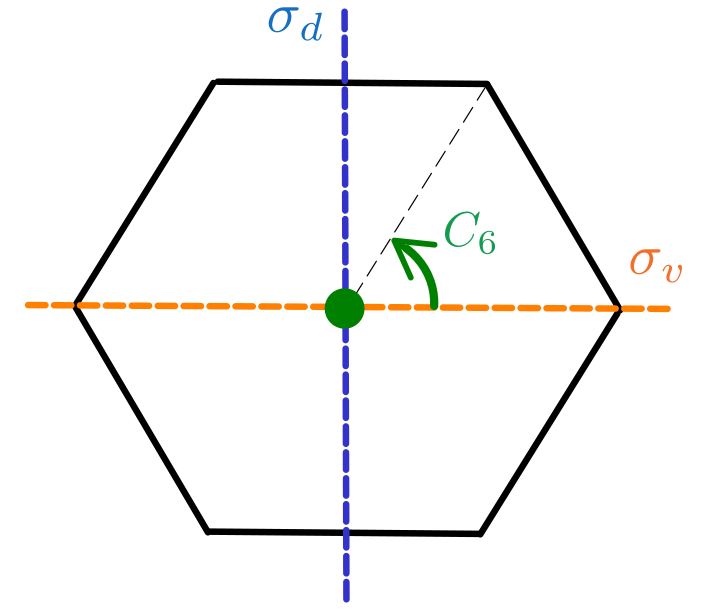
\includegraphics[width=0.4\linewidth]{fig/hexagon.png}
\caption{2D spatial symmetries of a hexagon.}
\label{fig:hexagon}
\end{figure}

\begin{example} \label{ex:symm_elems_hexagon_D6_example}
In a certain sense, a basic hexagon has 12 symmetry elements. Looking at Figure \ref{fig:hexagon}, the hexagon has the reflections $\sd$, $\sv$, the $60^\circ$ rotation $\Cs$, and all the combinations of these. Combining all the possibilities, we say all that the symmetry elements of the hexagon form the \textit{group}
\begin{equation} \label{eq:all_D6_elements}
D_6 = \{E, \Cs, \underbrace{\Ct}_{\Csn{2}}, \underbrace{C_2}_{\Csn{3}}, \underbrace{\Ctn{2}}_{\Csn{4}}, \Csn{5}, \sd, \underbrace{\sdp}_{\sd \Ct}, \underbrace{\sdpp}_{\sd \Ctn{2}}, \sv, \underbrace{\svp}_{\sv \Ct}, \underbrace{\svpp}_{\sv \Ctn{2}} \}.
\end{equation}
In this list, we did not include repeated elements, observe that $\Csn{6} = \sdn{2} = \svn{2} = E$ is the element the identity element, the one that ``does nothing''.
\end{example}


The concept of \textit{group} $G$ grasps the set of elements $a \in G$ that represent the symmetry of an object, along with its symmetry operation ``$\vdot$''. The element $a \vdot b$ represents the ``composition'' of applying first the operation $a$, and then $b$.

\begin{definition}[\textbf{Group}] \label{def:group}
Given a set $G$ and a binary operation ``$\vdot$''$:G\times G \to G$, \textbf{the pair} $(G, \vdot)$ is called a \textit{group} if it satisfies the following properties:
\begin{enumerate}
\item (closure): $a \vdot b \in G$, for every $a, b \in G$.
\item (associativity): $(a \vdot b) \vdot c =  a \vdot (b \vdot c)$, for every $a, b, c \in G$.
\item (identity): There exists an (identity) element $E \in G$ such that $E \vdot a = a \vdot E = a$, for every $a \in G$.
\item (inverse): For every $a \in G$, there is (an inverse) $a^{-1} \in G$ such that $a \vdot a^{-1} = a^{-1} \vdot a = E$.
\end{enumerate}
\end{definition}
Normally in the literature, one speaks of the set $G$ as being ``the group'' instead of the pair $(G, \vdot)$ and omits the operation symbol ``$\vdot$'', simply writing $ab$ instead of $a \vdot b$. This is for convenience but, mathematically, the operation ``$\vdot$'' is crucial to define a group.

\begin{definition}[\textbf{Order}] \label{def:group_order}
Given any set $A$, we denote its number of elements by $\abs{A}$. The \textit{order} of a group $G$ is defined simply as its number of elements $\abs{G}$.
\end{definition}

\begin{example} \label{ex:subgroup_example_D3D6}
Frequently, an object $A$ has all the symmetries of another object $B$. In Figure \ref{fig:hexagon_subgroup}, the \textcolor{ForestGreen}{green hexagon} has all the symmetries of the \textcolor{Cyan}{cyan triangle}. The symmetry elements of the triangle form the group $D_3 = \{E, \Ct, \Ctn{2}, \sv, \svp, \svpp\}$. Because $D_3$ is a subset of $D_6$ and also forms a group by itself, we say that $D_3$ is a subgroup of $D_6$.
\end{example}

\begin{figure}[H]
\centering
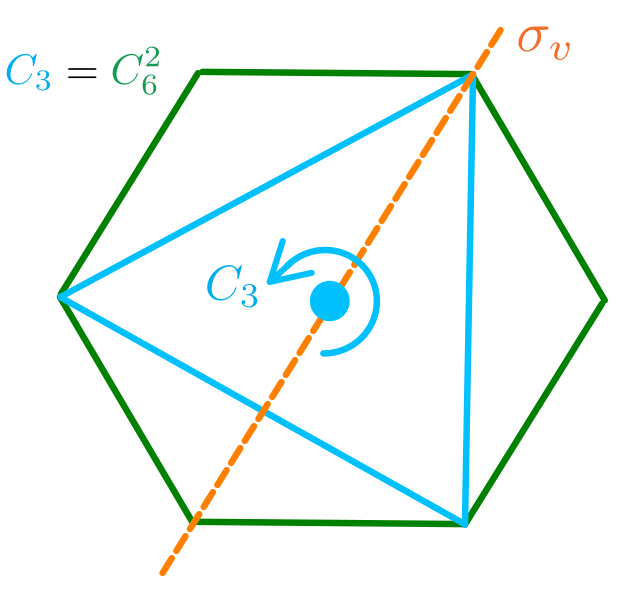
\includegraphics[width=0.4\linewidth]{fig/hexagon_subgroup.png}
\caption{The \textcolor{ForestGreen}{hexagon} has all the symmetries of the \textcolor{Cyan}{triangle}, i.e., $D_3$ is a subgroup of $D_6$.}
\label{fig:hexagon_subgroup}
\end{figure}


\begin{definition}[\textbf{Subgroup}] \label{def:subgroup}
If $(G, \vdot)$ is a group and $H$ is a subset of $G$, we say that $H$ is a subgroup of $G$ if the pair $(H, \vdot)$ is a group by itself.
\end{definition}

It is common that one defines a group by its \textit{generators}. We did that when defining the groups $D_6$ and $D_3$ associated to the hexagon and triangle, respectively at Figures \ref{fig:hexagon} and \ref{fig:hexagon_subgroup}. By generators, we mean:

\begin{definition}[\textbf{Generators of a group}] \label{def:generators_of_group}
If $S$ is a subset of a group $G$, we define $\ev{S}$ as the smallest subgroup of $G$ containing every element of $S$. The subgroup $\ev{S}$ is called the \textit{subgroup generated by $S$}. If $\ev{S} = G$, we say that the set $S$ \textit{generates} $G$.
\end{definition}


\begin{example} \label{ex:generators_example}
An intuitive way of thinking of $\ev{S}$ is by ``recursively multiplying'' all the elements of $S$, until all the possibilities are exhausted. In general for two elements:
\begin{equation} \label{eq:generate_two_elements}
\ev{\{a,b\}} = \{E, a, b, a^2, ab, ba, b^2, a^3, a^2b, aba, ba^2, ab^2, bab, b^2a, b^3, \ldots\}.
\end{equation}

For the hexagon at Figure \ref{fig:hexagon}, the set $\{\Cs, \sd, \sv\}$ generates the group $D_6$; and for the triangle at Figure \ref{fig:hexagon_subgroup}, the set $\{\Ct, \sv\}$ generates the group $D_3$.
\end{example}


\begin{definition}[\textbf{Cosets}] \label{def:left_cosets}
Let $G$ be a group and $H$ one of its subgroups. Given an element $g \in G$, we define the set $gH$ by
\begin{equation} \label{eq:gH_left_coset}
gH = \{g h \mid h \in H\} \subseteq G.
\end{equation}
This set $gH$ is called a \textit{left coset} of $G$ with respect to $H$, and $g$ is a \textit{representative} of $gH$. We denote the set of left cosets of $H$ by
\begin{equation} \label{eq:G/H_left_cosets}
G/H = \qty{gH \subseteq G \mid g \in G}.
\end{equation}

It is always possible to decompose $G$ as a disjoint union of its left cosets:
\begin{equation} \label{eq:disjoint_union_leftcosets}
G = \bigcup_{j=1}^{\abs{G/H}} g_j H = \sum_{j=1}^{\abs{G/H}} g_j H,
\end{equation}
where \( g_j \in G \) is a representative of the coset \( g_j H \), and \( \abs{G/H} \) denotes the number of distinct left cosets, also referred to as the \textit{index} of \( H \) in \( G \).
\end{definition}

An iconic theorem due to Laplace says that the order of a subgroup $H \subseteq G$ divides the order of the group $G$.

\begin{theorem}[\textbf{Laplace}]
The number of different left cosets is given by $\abs{G/H} = \abs{G} / \abs{H}$.
\end{theorem}

\begin{example} \label{ex:coset_decomp_D3D6}
As an example, take $H = D_3$ and $G = D_6$. We have that $\abs{D_3}=6$ and $\abs{D_6} = 12$. Therefore, we only have two different left cosets. One of them has $E$ as its representative:
\begin{equation} \label{eq:ED3-D6-first_coset}
E D_3 = D_3 = D_3 = \{E, \Ct, \Ctn{2}, \sv, \svp, \svpp\}.
\end{equation}

The other one is what is left of $D_6$, which has $\sd$ as its representative:
\begin{equation} \label{eq:sdD3-D6-second_coset}
\sd D_3 = \{\sd E, \sd \Ct, \sd \Ctn{2}, \sd \sv, \sd \svp, \sd \svpp\}
= \{ \sd, \sdp, \sdpp, C_2, \Csn{5}, \Cs \},
\end{equation}

The coset decomposition is the disjoint union of the two cosets
\begin{equation} \label{eq:D6_coset_decomp}
D_6 = ED_3 \cup \sd D_3.
\end{equation}
\end{example}

One would probably notice that the elements $\sd, \sdp, \sdpp$ are in some way related, also as $\sv, \svp, \svpp$. Actually, they belong to the same conjugacy class, which is a concept analogous to the notion of matrix similarity in Linear Algebra.

\begin{definition}[\textbf{Conjugacy class}] \label{def:conj_class}
Let \(G\) be a group and \(a, g, g' \in G\). If \(g' = aga^{-1}\), we say that \(g'\) is the \textit{conjugate} of \(g\) by \(a\), denoted as \(g' \sim g\). The set
\begin{equation} \label{eq:defi_conjclass_[g]}
[g] = \{ g' \in G \mid g' \sim g \} = \{ a g a^{-1} \mid a \in G \} \subseteq G
\end{equation}
is said to be a \textit{conjugacy class} (or simply a \textit{class}) of \(G\). Every group can be expressed as a disjoint union of its conjugacy classes.
\end{definition}

\begin{example} \label{ex:conjclass_example_D3D6}
For the groups $D_3$ and $D_6$, one finds the conjugacy classes

\begin{equation} \label{eq:D3_classes}
D_3 = [E] \cup [\Ct] \cup [\sv] = \{E\} \cup \{\Ct, \Ctn{2}\} \cup \{\sv, \svp, \svpp\},
\end{equation}
\begin{align} \label{eq:D6_classes}
D_6 &= \{E\} &&\cup&& \{C_2\} &&\cup&& \{\Ct, \Ctn{2}\} &&\cup&& \{\Cs, \Csn{5}\} &&\cup&& \{\sv, \svp, \svpp\} &&\cup&& \{\sd, \sdp, \sdpp\}.
\end{align}
\end{example}

\begin{example} \label{ex:homomorphism_sublattice_AB_example}
Let us say we want to identify which elements of $D_6$ exchange sublattice types $A$ and $B$, as in Figure \ref{fig:hexagon_AB}. We can accomplish this task by using a labelling function $\vphi: D_6 \to \{1, -1\}$, where
\begin{align} \label{eq:homomorphism_example_sublattices_AB_D6}
\vphi(g) =
\begin{cases}
\; \P1, \quad g \text{ changes sublattice type } A \leftrightarrow B, \\
\; -1, \quad \text{otherwise.}
\end{cases}
\end{align}

For our generators of $D_6$ we have $\vphi(\Cs) = -1$, $\vphi(\sv) = 1$ and $\vphi(\sd) = -1$. Only these values are sufficient, because if we treat $\{1, -1\}$ as a group by itself, with standard multiplication as its operation, one may notice that $\vphi$ follows the rule
\begin{equation} \label{eq:vphi_g1g2_homomophism}
\vphi(g_1 g_2) = \vphi(g_1) \vphi(g_2).
\end{equation}

The element $g_1 g_2$ changes sublattice only if exactly one of $g_1$ or $g_2$ do. Now, the elements $D_3$ do not exchange sublattice type, which translates to the property $\vphi(g) = 1$ for every $g \in D_3$.
\end{example}

\begin{figure}[H]
\centering
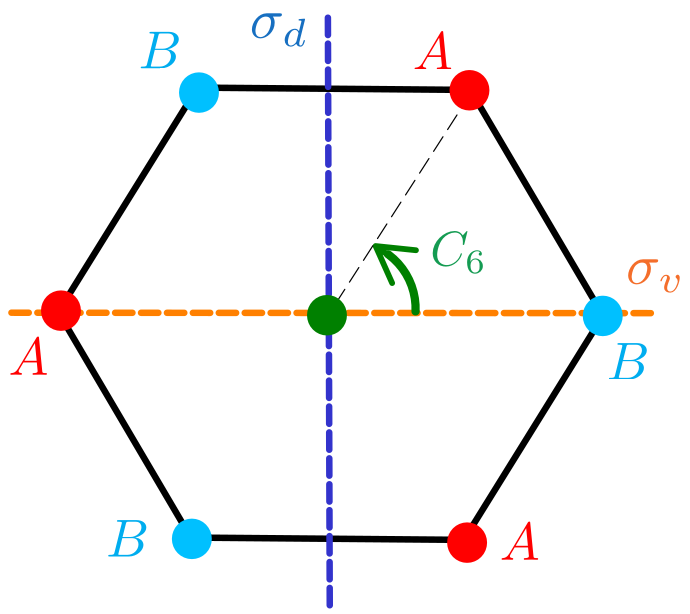
\includegraphics[width=0.4\linewidth]{fig/hexagon_AB.png}
\caption{Symmetries of \(D_6\) and the conventional sublattices \(A\) and \(B\) in graphene.}
\label{fig:hexagon_AB}
\end{figure}



The function $\vphi$ is generally known as a homomorphism, which in the case above identifies the subgroup $D_3$ as its kernel.

\begin{definition}[\textbf{Homomorphism}] \label{def:homomorphism}
Let $G$ and ${G'}$ be groups. A function $\vphi: G \to {G'}$ is called an \textit{homomorphism} if it preserves the group structure, i.e.,
\begin{equation} \label{eq:homomorphism}
\vphi(a b) = \vphi(a) \vphi(b), \quad \forall \, a,b \in G.
\end{equation}
If $\vphi$ is bijective, we also call it an \textit{isomorphism}. The kernel of $\vphi$ is defined as the set
\begin{equation} \label{eq:kernel_homomorphism}
\ker(\vphi) = \qty{g \in G \mid \vphi(g) = e_{G'}},
\end{equation}
where $e_{G'}$ is the identity element of ${G'}$.
\end{definition}

%%%%%%%%%%%%%%%%%%%%%%%%%%%%%%%%%%%%%%%%%%%%%%%%%%%%%%%%%%%%%%%%%%%%%%%%%%%%%%%%%%%%%%%%%%%%%%%%%%
\section{Elements of Representation Theory} \label{sec:representation_theory}
%%%%%%%%%%%%%%%%%%%%%%%%%%%%%%%%%%%%%%%%%%%%%%%%%%%%%%%%%%%%%%%%%%%%%%%%%%%%%%%%%%%%%%%%%%%%%%%%%%

In physics, specially in Quantum Mechanics, it is most common that one works with groups of matrices, where all the useful theorems of Functional Analysis hold.

\begin{definition}[\textbf{Groups of matrices}] \label{def:groups_of_matrices}
The set of invertible linear operators of a vector space $V$ form a group and we call it the \textit{general linear group}
\begin{equation} \label{eq:general_linear_GL(V)}
\GL(V) = \qty{A: V \to V \mid A \text{ is linear and invertible}}.
\end{equation}
If $V$ is finite dimensional with a scalar product, the set of unitary operators of $V$ is a subgroup of $\GL(V)$, defined by
\begin{equation} \label{eq:unitary_operators_U(V)}
\U(V) = \qty{A \in \GL(V) \mid A A^\dagger = \1}.
\end{equation}
%When $V = \mathbb{R}^n$ or $\C^n$, we can choose a basis and explicitly say that
%\begin{equation} \label{eq:GL(n)_defi}
%\GL(n, \mathbb{R}) = \qty{\text{invertible } n\times n \text{ real matrices}}, \;
%\GL(n, \mathbb{C}) = \qty{\text{invertible } n\times n \text{ complex matrices}}.
%\end{equation}
%In this case, the subgroups of orthogonal and unitary matrices are, respectively,
%\begin{equation} \label{eq:O(n)_defi}
%O(n) = \qty{A \in \GL(n, \mathbb{R}) \mid A A^T = \1}, \quad SO(n) = \qty{A \in O(n) \mid \det A = 1};
%\end{equation}
%\begin{equation} \label{eq:U(n)_defi}
%\U(n) = \qty{A \in \GL(n, \mathbb{C}) \mid A A^\dagger = \1}, \quad S\U(n) = \qty{A \in \U(n) \mid \det A = 1}.
%\end{equation}
\end{definition}

\begin{example} \label{ex:2x2_rep}
A group of $2\times 2$ matrices isomorphic to $D_3$ can be found by defining the homomorphism (representation) $\Gamma_2$ below
\begin{equation} \label{eq:D6_generators_2x2matrices}
\Gamma_2(\Ct) =
\begin{pmatrix}
\cos{\frac{2\pi}{3}} & \sin{\frac{2\pi}{3}} \\
-\sin{\frac{2\pi}{3}} & \cos{\frac{2\pi}{3}}
\end{pmatrix},
%\quad
%\Gamma_2(\sd) =
%\begin{pmatrix}
%-1 & 0 \\
%0 & 1
%\end{pmatrix},
\quad
\Gamma_2(\sv) =
\begin{pmatrix}
1 & 0 \\
0 & -1
\end{pmatrix}.
\end{equation}

Imposing the relation \ref{eq:homomorphism}, the other representative $2\times 2$ matrices $\Gamma_2(E), \Gamma_2(\Ctn{2}), \Gamma_2(\svp), \Gamma_2(\svpp)$ can be found by multiplying the matrices of the two generators in Equation \ref{eq:D6_generators_2x2matrices}.
\end{example}

\begin{definition}[\textbf{Representation}] \label{def:representation}
A \textit{representation} of a group $G$ on a vector space $V$ is a \textbf{homomorphism} $\Pi: G \to \GL(V)$.
\end{definition}

When applying the theory of representations to Quantum Mechanics, two key physical considerations must be incorporated. The first is the ability to change coordinate systems, and the second is the requirement to preserve probabilities by ensuring the unitarity of transformations.

\n

1. Conjugating an observable $H$ by means of $A$, as in $H' = A H A^{-1}$, corresponds to a change of reference frame (or basis). This leads us to regard two conjugate representations as equivalent, as they describe the same transformation in different bases.

\begin{definition}[\textbf{Equivalent representations}] \label{def:equiv_representations}
Two representations $\Pi_1: G \to \GL(V_1)$ and $\Pi_2: G \to \GL(V_2)$ of a group $G$ are said to be \textit{equivalent} if there is an invertible linear operator $A: V_1 \to V_2$ such that
\begin{equation} \label{eq:intertwiner}
\Pi_2(g) = A \Pi_1(g) A^{-1}, \, \forall \, g \in G.
\end{equation}
In this case we write $\Pi_1 \equiv \Pi_2$.
\end{definition}

2. In Quantum Mechanics, unitary matrices are standard because they preserve probabilities and ensure the physical consistency of the theory. Moreover, as we will see in Section \ref{sec:characters}, unitary representations are particularly significant due to the orthogonality theorems for representation characters, which fundamentally depend on this restriction. Lastly, this preference for unitary representations is not merely practical but is underpinned by the general principle stated in Theorem \ref{th:unitarity_rep} \cite{dresselhaus}.

\begin{theorem}[\textbf{Unitarity of representations}] \label{th:unitarity_rep}
A representation $\Gamma: G \to \GL(V)$ is called \textit{unitary} if $\Gamma(g) \in \U(V)$, $\forall \, g \in G$. Every representation $\Pi: G \to \GL(V)$ is equivalent to some unitary representation $\Gamma: G \to \U(V)$.
\end{theorem}

Because of Theorem \ref{th:unitarity_rep}, most of our theory will be dedicated to unitary representations. If not otherwise stated, when we consider a representation we actually mean an \textbf{unitary representation}.

\begin{example} \label{ex:direct_sum}
Considering $G = D_3$, take $\Gamma_2$ acting on $V_2 = \mathbb{R}^2$, as previously defined in Example \ref{ex:2x2_rep}, and also consider the trivial representation $\Gamma_1$ acting on $V_1 = \mathbb{R}$, which is defined by $\Gamma_1(g) = 1$, $\forall \, g \in G$. We can stack $\Gamma_2$ and $\Gamma_1$ to construct another representation $\Gamma$, acting on $V_2 \oplus V_1$, given by
\begin{equation} \label{eq:block_diagonal_Gamma_2_1}
\Gamma(g) =
\begin{pmatrix}
\Gamma_2(g) & 0 \\
0 & \Gamma_1(g)
\end{pmatrix}, \quad \forall \, g \in G.
\end{equation}
\begin{equation} \label{eq:D6_generators_3x3matrices}
\Gamma(\Ct) =
\begin{pmatrix}
\cos{\frac{2\pi}{3}} & \sin{\frac{2\pi}{3}} & 0 \\
-\sin{\frac{2\pi}{3}} & \cos{\frac{2\pi}{3}} & 0 \\
0 & 0 & 1
\end{pmatrix},
%\;
%\Gamma(\sd) =
%\begin{pmatrix}
%-1 & 0 & 0 \\
%0 & 1 & 0 \\
%0 & 0 & 1
%\end{pmatrix},
\quad
\Gamma(\sv) =
\begin{pmatrix}
1 & 0 & 0 \\
0 & -1 & 0 \\
0 & 0 & 1
\end{pmatrix}.
\end{equation}

We say that $\Gamma$ is a direct sum and we write $\Gamma \equiv \Gamma_2 \oplus \Gamma_1$. Representations, such as $\Gamma$, that can be decomposed into a direct sum are called \textit{reducible}. What distinguishes reducible representations is the existence of nontrivial invariant subspaces.
\end{example}

\begin{definition}[\textbf{Invariant subspace}] \label{def:invariant_subspace}
A vector subspace $W \subseteq V$ is said to be \textit{invariant} under a representation $\Pi: G \to \GL(V)$ if it satisfies $\Pi(g) W \subseteq W$ (the action of $\Pi(g)$ on $W$ is contained within $W$), for every $g \in G$.
\end{definition}

\begin{example} \label{ex:invariant_subspaces}
The nontrivial subspaces $V_2$ and $V_1$ are invariant under the action of $\Gamma$, defined in Example \ref{ex:direct_sum}. In Equation \ref{eq:block_diagonal_Gamma_2_1}, we see that $\Gamma(g)$ is block diagonal on subspaces $V_2$ and $V_1$, therefore we have that $\Gamma(g) V_2 \subseteq V_2$ and $\Gamma(g) V_1 \subseteq V_1$.
\end{example}

\begin{definition}[\textbf{Irreducible representation}] \label{def:irrep}
A representation $\Pi: G \to \GL(V)$ always has the trivial invariant subspace $\{0\}$ and $V$. If there are not others, $\Pi$ is said to be \textit{irreducible}.
\end{definition}

\begin{example} \label{ex:irrep_Gamma12_example}
Still in the context of Example \ref{ex:direct_sum}, unlike $\Gamma$, the representations $\Gamma_1$ and $\Gamma_2$ of $D_3$ are \textit{irreducible} because they have no trivial invariant subspaces and are not equivalent to any block diagonal representation.
\end{example}

Theorem \ref{th:irreps_decomp}, whose proof can be found in \cite{dresselhaus, hamermesh}, states that irreducible representations (irreps) are building blocks for all representations in finite dimensional vector spaces.

\begin{theorem}[\textbf{Decomposition of unitary representations}] \label{th:irreps_decomp}
Let $V$ be a finite dimensional vector space with a scalar product and let $\Gamma: G \to \U(V)$ be an unitary representation. Then, $\Gamma$ is either irreducible or reducible and can be decomposed into a direct sum
\begin{equation} \label{eq:decomp_unitary_reps}
V = \bigoplus_{j=1}^N V_j, \quad
\Gamma(g) =
\begin{pmatrix}
\Gamma_1(g) &  &  \\
 & \ddots &  \\
 &  & \Gamma_N(g) \\
\end{pmatrix},
\end{equation}
where each $V_j$ is a nontrivial invariant subspace under $\Gamma$ and $\Gamma_j: G \to \U(V_j)$ is an irreducible representation of $G$. To summarize this, we write $\Gamma \equiv \bigoplus_{j=1}^N \Gamma_j$.
\end{theorem}

%%%%%%%%%%%%%%%%%%%%%%%%%%%%%%%%%%%%%%%%%%%%%%%%%%%%%%%%%%%%%%%%%%%%%%%%%%%%%%%%%%%%%%%%%%%%%%%%%%
\subsection{Characters} \label{sec:characters}
%%%%%%%%%%%%%%%%%%%%%%%%%%%%%%%%%%%%%%%%%%%%%%%%%%%%%%%%%%%%%%%%%%%%%%%%%%%%%%%%%%%%%%%%%%%%%%%%%%

The trace of a representation is such an important quantity that it deserves the name of its \textit{character}. The \textit{characters} of irreps from a group provides enough information to determine the decomposition of a reducible representation into irreducible ones, as in Theorem \ref{th:irreps_decomp}.

\begin{definition}[\textbf{Character}] \label{def:character}
The \textit{character} of an element $g \in G$ in the representation $\Pi: G \to \GL(V)$ is defined as
\begin{equation} \label{eq:character}
\chi^{(\Pi)}(g) = \tr[\Pi(g)] = \sum_{j} \Pi_{jj}(g).
\end{equation}
\end{definition}

\begin{lemma} \label{lemma:character_equiv_sameclass}
Due to the cyclic property of the matrix trace, equivalent irreps \(\Pi\) and \(\Pi'\) share the same characters:
\begin{equation} \label{eq:trace_equivalent_reps_chi}
\Pi'(g) = A\Pi(g)A^{-1} \implies \chi^{(\Pi')}(g) = \tr[A \Pi(g) A^{-1}] =  \tr[A^{-1}A \Pi(g)] = \chi^{(\Pi)}(g).
\end{equation}

Elements \(g\) and \(g' = aga^{-1}\) belonging to the same conjugacy class also have the same character:
\begin{equation} \label{eq:trace_same_class_chi}
\chi(g') = \chi(aga^{-1}) = \tr[\Pi(aga^{-1})] = \tr[\Pi(a)\Pi(g)\Pi(a^{-1})] = \tr[\Pi(a)^{-1}\Pi(a)\Pi(g)] = \chi(g).
\end{equation}

As a result, we can define the character of a class \(S = [g]\), denoted by \(\chi_S = \chi(g) = \chi(g')\).
\end{lemma}

\n

Now we are going to state the ``Wonderful Orthogonality Theorems'' for characters, whose proof can be found in \cite{dresselhaus, hamermesh}. They will be useful to construct the character table of a group.

\begin{theorem}[\textbf{1st Wonderful Orthogonality Theorem}] \label{th:1st-wot}
The characters $\chi^{(\Gamma_i)}$, $\chi^{(\Gamma_j)}$ of irreducible representations $\Gamma_i, \Gamma_j: G \to \U(V)$ obey the orthogonality relation
\begin{equation} \label{eq:1st-wot}
\delta_{\Gamma_i, \Gamma_j} =
\frac{1}{\abs{G}} \sum_{g \in G} \chi^{(\Gamma_i)}(g) \chi^{(\Gamma_j)}(g)^* =
\frac{1}{\abs{G}} \sum_{S} \abs{S} \, \chi^{(\Gamma_i)}_S \qty[\chi^{(\Gamma_j)}_S]^*,
\end{equation}
where the sum in $S$ runs through the conjugacy classes of $G$, with $\abs{S}$ denoting the number of elements of the class $S$.
\end{theorem}

Let $n_{\text{classes}}$ be the number of different classes of $G$. If we fix an irrep $\Gamma_i$ and consider a $n_{\text{classes}} -$dimensional vector space, with vectors
\begin{equation} \label{eq:nclasses_space}
\ket{\psi^{(\Gamma_i)}} =
\qty(
\sqrt{\frac{\abs{S_1}}{\abs{G}}} \chi^{(\Gamma_i)}_{S_1},
\sqrt{\frac{\abs{S_2}}{\abs{G}}} \chi^{(\Gamma_i)}_{S_2},
\ldots,
\sqrt{\frac{\abs{S_m}}{\abs{G}}} \chi^{(\Gamma_i)}_{S_{n_{\text{classes}}}}
),
\end{equation}
Equation \ref{eq:1st-wot} can be rewritten as
\begin{equation} \label{eq:orthog_psis_irreps}
\braket{\psi^{(\Gamma_i)}}{\psi^{(\Gamma_j)}} = \delta_{\Gamma_i, \Gamma_j}.
\end{equation}

As a consequence, there are no more than $n_{\text{classes}}$ of such vectors. If there were more, they would be linearly dependent, contradicting Equation \ref{eq:orthog_psis_irreps}. From this, we conclude that the number of irreps satisfies $n_{\text{irreps}} \leq n_{\text{classes}}$.

\begin{theorem}[\textbf{2nd Wonderful Orthogonality Theorem}] \label{th:2nd-wot}
Let $\Gamma_j: G \to \U(V)$ be the irreducible representations of $G$. The summation over all irreps
\begin{equation} \label{eq:2nd-wot}
\delta_{S, S'} = \frac{1}{\abs{G}} \sum_{\Gamma_j} \abs{S} \, \chi^{(\Gamma_j)}_S \qty[\chi^{(\Gamma_j)}_{S'}]^*
\end{equation}
also yields an orthogonality relation, where $S$ and $S'$ are conjugacy classes of $G$.
\end{theorem}

\begin{corollary} \label{coro:chi_E}
Applying Theorem \ref{th:2nd-wot} to the trivial class $S = S' = \{E\}$ yields
\begin{equation} \label{eq:chi_E_coro}
\abs{G} = \sum_{\Gamma_j} \abs{\chi^{(\Gamma_j)}(E)}^2 = \sum_{\Gamma_j} \ell_j^2,
\end{equation}
where $\ell_j = \chi^{(\Gamma_j)}(E)$ is the dimension of the irrep $\Gamma_j$.
\end{corollary}

Analogous to Equation \ref{eq:nclasses_space} we can apply the same reasoning to a $n_{\text{irreps}}-$dimensional vector space. Fixing a class $S$ and considering the vectors
\begin{equation} \label{eq:nirreps_space}
\ket{\phi_{S}} =
\qty(
\sqrt{\frac{\abs{S}}{\abs{G}}} \chi^{(\Gamma_1)}_{S},
\sqrt{\frac{\abs{S}}{\abs{G}}} \chi^{(\Gamma_2)}_{S},
\ldots,
\sqrt{\frac{\abs{S}}{\abs{G}}} \chi^{\qty(\Gamma_{n_{\text{irreps}}})}_{S}
),
\end{equation}
Equation \ref{eq:2nd-wot} implies the orthogonality relation
\begin{equation} \label{eq:orthog_phis_classes}
\braket{\phi_{S}}{\phi_{S'}} = \delta_{S, S'}.
\end{equation}

As such, we also conclude that $n_{\text{classes}} \leq n_{\text{irreps}}$. This allows us to establish Theorem \ref{th:num_irreps_classes}.

\begin{theorem}[$\bm{n_{\textbf{irreps}} = n_{\textbf{classes}}}$] \label{th:num_irreps_classes}
The number of irreducible representations of a group $G$ is equal to its number of conjugacy classes.
\end{theorem}

With the orthogonality theorems \ref{th:1st-wot} and \ref{th:2nd-wot}, along with the fact that \(n_{\text{irreps}} = n_{\text{classes}}\), we can construct character tables. These tables provide complete information for decomposing any representation into irreducible ones. %In fields such as chemistry and crystallography, they are used to classify molecular vibrations according to their symmetry and to predict whether a transition between two states is forbidden by symmetry.

\begin{example} \label{ex:chartable_construction_D3}
In Example \ref{ex:direct_sum} we established two irreducible representations $\Gamma_1$ and $\Gamma_2$. From Equation \ref{eq:D3_classes}, the group $D_3$ has three distinct classes, and thus also three inequivalent irreducible representations. Calculating the characters under $\Gamma_1$ and $\Gamma_2$, we obtain
\begin{align} \label{eq:incomplete_characters_D3}
& \chi^{(\Gamma_1)}(E) = 1, && \chi^{(\Gamma_1)}(\Ct) = 1 , && \chi^{(\Gamma_1)}(\sv) = 1, \\
& \chi^{(\Gamma_2)}(E) = 2, && \chi^{(\Gamma_2)}(\Ct) = 2 \cos(\frac{2\pi}{3}) = -1, && \chi^{(\Gamma_2)}(\sv) = 0.
\end{align}

Using Corollary \ref{coro:chi_E}, we obtain for the third irrep $\Gamma_3$ that $6 = 2^2 + 1^2 + \ell_3^2 \implies \ell_3 = 1$,
which tells us $\Gamma_3$ is one-dimensional and its matrix representatives are numbers $\Gamma_3(g) = \chi^{(\Gamma_3)}(g)$.

Since \(\Ct^3 = E\) and \(\sv^2 = E\), it follows that \(\Gamma_3(\Ct)^3 = 1\) and \(\Gamma_3(\sv)^2 = 1\). We can immediately conclude that \(\Gamma_3(\Ct) = 1\). For \(\sv\), however, we must have \(\Gamma_3(\sv) = -1\), since if it were 1, we would obtain \(\Gamma_3 \equiv \Gamma_1\). Summarizing the results for \(\Gamma_3\), we have:
\begin{align} \label{eq:Gamma3_characters_D3}
\chi^{(\Gamma_3)}(E) = 1, && \chi^{(\Gamma_3)}(\Ct) = 1, && \chi^{(\Gamma_3)}(\sv) = -1.
\end{align}

With all irreps, classes and characters known, we construct the table of characters for $D_3$:

\vspace{-0.5em}

\begin{table}[H]
\caption{Character table of group $D_3$ (or $C_{3v}$).}
\centering
\begin{tabular} { c c c c }
\specialrule{0.05em}{0em}{0.2em}
$\P$ & $\P E$ & $\P 2 C_3$ & $\P 3 C_2'$ \\
\specialrule{0.01em}{0.2em}{0.2em}
$A_1$ & $\P1$ & $\P1$ & $\P1$ \\
\specialrule{0.01em}{0.2em}{0.2em}
$A_2$ & $\P1$ & $\P1$ & $ -1$ \\
\specialrule{0.01em}{0.2em}{0.2em}
$E$   & $\P2$ & $ -1$ & $\P0$ \\
\specialrule{0.05em}{0.2em}{0em}
\end{tabular}
\label{tab:D3}
\end{table}

\vspace{-0.5em}

In Table \ref{tab:D3}, we renamed the representations \(A_1 = \Gamma_1\), \(A_2 = \Gamma_3\), and \(A_3 = \Gamma_2\) to align with the standard notation commonly used in the literature. In the first row, the notation \(nA\) indicates a conjugacy class \([A]\) containing \(n\) elements. For instance, \(2C_3\) represents the conjugacy class \([C_3] = \{C_3, C_3^2\}\), which consists of two elements. %Additionally, it can be verified that the rows and columns of Table \ref{tab:D3} satisfy the orthogonality theorems \ref{th:1st-wot} and \ref{th:2nd-wot}.
\end{example}

An analogous procedure in Example \ref{ex:chartable_construction_D3} could be applied to construct the character table for the group $D_6$, which we show in Table \ref{tab:D6}.
\begin{table}[H]
\caption{Character table of group $D_6$ (or $C_{6v}$).}
\centering
\begin{tabular} { c c c c c c c  }
\specialrule{0.05em}{0em}{0.2em}
$\P$ & $\P E$ & $\P C_2$ & $\P2C_3$ & $\P2C_6$ & $\P3C_2'$ & $\P3C_2''$ \\
\specialrule{0.01em}{0.2em}{0.2em}
$A_1$ & $\P1$ & $\P1$ & $\P1$ & $\P1$ & $\P1$ & $\P1$ \\
\specialrule{0.01em}{0.2em}{0.2em}
$A_2$ & $\P1$ & $\P1$ & $\P1$ & $\P1$ & $ -1$ & $ -1$ \\
\specialrule{0.01em}{0.2em}{0.2em}
$B_1$ & $\P1$ & $ -1$ & $\P1$ & $ -1$ & $\P1$ & $ -1$ \\
\specialrule{0.01em}{0.2em}{0.2em}
$B_2$ & $\P1$ & $ -1$ & $\P1$ & $ -1$ & $ -1$ & $\P1$ \\
\specialrule{0.01em}{0.2em}{0.2em}
$E_1$ & $\P2$ & $ -2$ & $ -1$ & $\P1$ & $\P0$ & $\P0$ \\
\specialrule{0.01em}{0.2em}{0.2em}
$E_2$ & $\P2$ & $\P2$ & $ -1$ & $ -1$ & $\P0$ & $\P0$ \\
\specialrule{0.05em}{0.2em}{0em}
\end{tabular}
\label{tab:D6}
\end{table}

With the information from the character tables, we can decompose a representation into irreducible components using Theorem \ref{th:reduction_formula}, the proof of which is detailed in \cite{dresselhaus, hamermesh}.

\begin{theorem}[\textbf{Reduction formula}] \label{th:reduction_formula}
By Theorem \ref{th:irreps_decomp}, a representation $\Gamma: G \to \U(V)$ is a direct sum of irreps
\begin{equation} \label{eq:Gamma_direct_sum_of_irreps}
\Gamma \equiv \bigoplus_j r_j \, \Gamma_j,
\end{equation}
where the coefficients $r_j \in \N_{>0}$ denote the number of times the irrep $\Gamma_j$ appears in the decomposition of $\Gamma$. The coefficients $r_j$ are given by the \textit{reduction formula}
\begin{equation} \label{eq:reduction_formula}
r_j =
\frac{1}{\abs{G}} \sum_{g \in G} \chi^{(\Gamma)}(g) \chi^{(\Gamma_j)}(g)^* =
\frac{1}{\abs{G}} \sum_{S} \abs{S} \, \chi^{(\Gamma)}_S \qty[\chi^{(\Gamma_j)}_S]^*.
\end{equation}
\end{theorem}

If two unitary representations \(\Pi_1\) and \(\Pi_2\) have identical characters for each conjugacy class, then, by Equation \ref{eq:reduction_formula}, the coefficients \(r_j\) for both \(\Pi_1\) and \(\Pi_2\) are identical. Consequently, the representations are equivalent.
\begin{equation} \label{eq:Phi_Psi_rj_equivalent}
\Pi_1 \equiv \bigoplus_j r_j \, \Gamma_j \equiv \Pi_2.
\end{equation}
Conversely, as established in Lemma \ref{lemma:character_equiv_sameclass}, equivalent representations share the same characters. Together, these results lead to the following statement:

\begin{corollary} \label{coro:same_characters_equiv_reps}
Two unitary representations are equivalent if and only if they have the same characters for every conjugacy class.
\end{corollary}


%%%%%%%%%%%%%%%%%%%%%%%%%%%%%%%%%%%%%%%%%%%%%%%%%%%%%%%%%%%%%%%%%%%%%%%%%%%%%%%%%%%%%%%%%%%%%%%%%%
\subsection{Induction and subduction of representations} \label{sec:induction_subsuction}
%%%%%%%%%%%%%%%%%%%%%%%%%%%%%%%%%%%%%%%%%%%%%%%%%%%%%%%%%%%%%%%%%%%%%%%%%%%%%%%%%%%%%%%%%%%%%%%%%%

\begin{definition}[\textbf{Subduction}] \label{def:subduction_defi}
Let $H \subseteq G$ be a subgroup and $\Pi: G \to \GL(V)$ a representation of $G$. We can naturally construct of a representation $\rho: H \to \GL(V)$ of $H$ on $V$ by restricting $\Pi$ to elements of $H$:
\begin{equation} \label{eq:subduction_defi}
\rho(h) = \Pi(h), \quad \forall \, h \in H \subseteq G.
\end{equation}
We denote $\rho = \Pi \downarrow H$ and is called the \textit{subduction} of $\Pi$ to the subgroup $H$.
\end{definition}

\begin{example} \label{ex:C3_D3_subduction_example}
$H = \{E, \Ct, \Ctn{2}\} \subseteq G = D_3$ and $\Pi = \Gamma_2$ as defined in Example \ref{ex:2x2_rep}. The subduced representation $\rho = \Pi \downarrow H$ is obtained by using the matrices $\Pi(h)$, for $h = E, \Ct, \Ctn{2}$.
\begin{equation} \label{eq:rho_subduced_C3_D3_subduction_example}
\rho(E) =
\begin{pmatrix}
1 & 0 \\
0 & 1
\end{pmatrix},
\quad
\rho(\Ct) =
\begin{pmatrix}
\cos(\frac{2\pi}{3}) & \sin(\frac{2\pi}{3}) \\
-\sin(\frac{2\pi}{3}) & \cos(\frac{2\pi}{3})
\end{pmatrix},
\quad
\rho(\Ctn{2}) =
\begin{pmatrix}
\cos(\frac{4\pi}{3}) & \sin(\frac{4\pi}{3}) \\
-\sin(\frac{4\pi}{3}) & \cos(\frac{4\pi}{3})
\end{pmatrix}.
\end{equation}

The original representation \(\Pi\) includes additional matrices not present in \(\rho\):
\begin{equation} \label{eq:Pi_C3_D3_subduction_example}
\Pi(\sv) =
\begin{pmatrix}
1 & 0 \\
0 & 1
\end{pmatrix},
\;
\Pi(\svp) = \Pi(\sv \Ct) =
\begin{pmatrix}
-\frac{1}{2} & \frac{\sqrt{3}}{2} \\
\frac{\sqrt{3}}{2} & \frac{1}{2}
\end{pmatrix},
\;
\Pi(\svpp) = \Pi(\sv \Ctn{2}) =
\begin{pmatrix}
-\frac{1}{2} & -\frac{\sqrt{3}}{2} \\
-\frac{\sqrt{3}}{2} & \frac{1}{2}
\end{pmatrix},
\end{equation}
As discussed in Example \ref{ex:irrep_Gamma12_example}, \(\Pi = \Gamma_2\) is irreducible because its six matrices cannot be transformed into block diagonal form through any conjugate transformation \(A \Pi(g) A^{-1}\), \(\forall g \in D_3\).

However, if we consider only the three matrices in Equation \ref{eq:rho_subduced_C3_D3_subduction_example}, they can be transformed into block diagonal form through the following conjugation by \(A\):
\begin{equation} \label{eq:subduction_can_be_reducible_example}
\rho(E) =
A
\begin{pmatrix}
1 & 0 \\
0 & 1
\end{pmatrix}
A^{-1},
\quad
\rho(\Ct) =
A
\begin{pmatrix}
e^{-\frac{2\pi i}{3}} & 0 \\
0 & e^{\frac{2\pi i}{3}}
\end{pmatrix}
A^{-1},
\quad
\rho(\Ctn{2}) =
A
\begin{pmatrix}
e^{-\frac{4\pi i}{3}} & 0 \\
0 & e^{\frac{4\pi i}{3}}
\end{pmatrix}
A^{-1},
\quad
\end{equation}
\begin{equation} \label{eq:A_matrix_that_diagonalizes}
A =
\begin{pmatrix}
i & -i \\
1 & 1
\end{pmatrix}.
\end{equation}
Therefore, we can assert that \(\rho\) is a direct sum of two one-dimensional representations, \(\{1, e^{-\frac{2\pi i}{3}}, e^{-\frac{4\pi i}{3}}\}\) and \(\{1, e^{\frac{2\pi i}{3}}, e^{\frac{4\pi i}{3}}\}\), making it reducible. This demonstrates that the subduction of an irreducible representation can result in a reducible one.

\end{example}

The inverse process of subduction, known as \textit{induction}, is more complex. It involves starting with a representation \(\Pi\) of \(H\) and constructing a corresponding representation for the larger group \(G\).

\begin{definition}[\textbf{Induction}] \label{def:induction_defi}
Let $H$ be a subgroup of a finite group $G$ and $\Pi: H \to \GL(V)$ be a representation of $H$ on a $n$-dimensional vector space $V$. Let $R = \{g_1, \ldots, g_m\} \subseteq G$ be a full set of representatives of the left cosets in $G/H$, where $m = \abs{G/H}$. Consider the following $(m\cdot n)$-dimensional vector space
\begin{equation} \label{eq:W_vectorspace_induction_copies}
W = \bigoplus_{i=1}^m g_i V = \qty{w = \bigoplus_{i=1}^n (g_i, v_i) \;\bigg|\; v_i \in V_i},
\end{equation}
where each $g_i V$ is an isomorphic labelled copy of $V$, defined by
\begin{equation} \label{eq:giV_vectorspace_labelled_copy}
g_i V = \{ (g_i, v) \mid g_i \in G, v \in V\}, \quad
\alpha (g_i, u) + \beta (g_i, v) = (g_i, \alpha u + \beta v).
\end{equation}

For each $g \in G$ and $g_i \in R$ there is an $h_i \in H$ and a permutation index $j(i) \in \{1, \ldots, m\}$ such that $g g_i = g_{j(i)} h_i$. The \textit{induced} representation $\rho: G \to \GL(W)$, denoted by $\rho = \Pi \uparrow G$, is defined by the action on an element $w = \bigoplus_{i=1}^{m} (g_i, v_i) \in W$:
\begin{equation} \label{eq:induced_rep_action_defi}
\rho(g) w = \bigoplus_{i=1}^{m} \qty(g_{j(i)}, \Pi(h_i) v_i) \in W.
\end{equation}
\end{definition}

\begin{example} \label{ex:induced_rep_C3D3}
$H = \{E, \Ct, \Ctn{2}\}$, $G = D_3$ and $\Pi$ is an one-dimensional representation of $H$ (on vector space $\C^1$), defined by $\Pi(E) = 1$, $\Pi(\Ct) = e^{\frac{2\pi i}{3}}$, $\Pi(\Ctn{2}) = e^{\frac{4\pi i}{3}}$.

\n

Take $R = \{g_1 = E, g_2 = \sv\}$, where we have the coset decomposition
\begin{equation} \label{eq:coset_decomp_of_D3_subgroup_C3}
D_3 = \bigcup_{g_i \in R} g_i H =
E H \cup \sv H = \{E, \Ct, \Ctn{2}\} \cup \{\underbrace{\sv}_{\sv E}, \underbrace{\svp}_{\sv \Ct}, \underbrace{\svpp}_{\sv \Ctn{2}}\}.
\end{equation}

Let us calculate the actions of $\rho = \Pi \uparrow G$ on the generators $\{\Ct, \sv\}$ of $D_3$.

$g = \Ct$:

$g_1 = E \implies g g_1 = \Ct E = E \Ct = g_1 h_1$, where $j(1) = 1$ and $h_1 = \Ct$.

$g_2 = \sv \implies g g_2 = \Ct \sv = \svpp = \sv \Ctn{2} = g_2 h_2$, where $j(2) = 2$ and $h_2 = \Ctn{2}$.

\n

On the basis $(w_{11}, w_{21})$, where $w_{ij} = (g_i, e_j)$ and $(e_1)$ is the basis of $\C^1$, we have
\begin{equation} \label{eq:rhoC3_w11_example_inducedrep_C3D3}
\rho(\Ct) w_{11} = (g_{j(1)}, \Pi(h_1) e_1) = \qty(g_1, e^{\frac{2\pi i}{3}} e_1) = e^{\frac{2\pi i}{3}} w_{11}
\end{equation}
\begin{equation} \label{eq:rhoC3_w21_example_inducedrep_C3D3}
\rho(\Ct) w_{21} = (g_{j(2)}, \Pi(h_2) e_1) = \qty(g_2, e^{\frac{4\pi i}{3}} e_1) = e^{\frac{4\pi i}{3}} w_{21}
\end{equation}
\begin{equation} \label{eq:rhoC3_matrix_example_inducedrep_C3D3}
\boxed{ \rho(\Ct) =
\begin{pmatrix}
e^{\frac{2\pi i}{3}} & 0 \\
0 & e^{\frac{4\pi i}{3}}
\end{pmatrix} } =
\begin{pmatrix}
\Pi\qty(h_1) & 0 \\
0 & \Pi(h_2)
\end{pmatrix} =
\begin{bmatrix}
\Pi(g_{j(1)}^{-1} \Ct g_1) & 0 \\
0 & \Pi(g_{j(2)}^{-1} \Ct g_2)
\end{bmatrix}.
\end{equation}

\n

$g = \sv$:

$g_1 = E \implies g g_1 = \sv E = g_2 h_1$, where $j(1) = 2$ and $h_1 = E$.

$g_2 = \sv \implies g g_2 = \sv \sv = E = E E = g_1 h_2$, where $j(2) = 1$ and $h_2 = E$.

\begin{equation} \label{eq:rhoC3_w11_example_inducedrep_C3D3}
\rho(\sv) w_{11} = (g_{j(1)}, \Pi(h_1) e_1) = \qty(g_2, e_1) = w_{21}
\end{equation}
\begin{equation} \label{eq:rhoC3_w21_example_inducedrep_C3D3}
\rho(\sv) w_{21} = (g_{j(2)}, \Pi(h_2) e_1) = \qty(g_1, e_1) = w_{11}
\end{equation}
\begin{equation} \label{eq:rhoC3_matrix_example_inducedrep_C3D3}
\boxed{ \rho(\sv) =
\begin{pmatrix}
0 & 1 \\
1 & 0
\end{pmatrix} } =
\begin{pmatrix}
0 & \Pi\qty(h_2) \\
\Pi\qty(h_1) & 0
\end{pmatrix} =
\begin{bmatrix}
0 & \Pi(g_{j(2)}^{-1} \sv g_2) \\
\Pi(g_{j(1)}^{-1} \sv g_1) & 0
\end{bmatrix}.
\end{equation}

The induced representation \(\rho\) is two-dimensional, with characters \(\chi^{(\rho)}(E) = 2\), \(\chi^{(\rho)}(\Ct) = -1\), and \(\chi^{(\rho)}(\sv) = 0\). By Corollary \ref{coro:same_characters_equiv_reps}, we conclude that the induced representation \(\rho\) is equivalent to the irreducible representation \(E\) from Table \ref{tab:D3}.

\end{example}

\begin{example} \label{ex:induced_rep_D3D6}
Take $G = D_6$, $H = D_3$ and $\Pi = \Gamma_2: H \to \GL(\mathbb{R}^2)$ from Example \ref{ex:2x2_rep}. Using the coset decomposition of $D_6$ from Example \ref{ex:coset_decomp_D3D6}, we obtain the set of coset representatives $R = \{g_1=E, g_2=\sd\}$. Let us calculate the actions of $\rho = \Pi \uparrow G$ for the generators $\{\Cs, \sd, \sv\}$.

\n

$g = \Cs$:

$g_1 = E \implies g g_1 = \Cs E = \Cs = \sd \svpp = g_2 h_1$, where $j(1) = 2$ and $h_1 = \svpp$.

$g_2 = \sd \implies g g_2 = \Cs \sd = \svp = E \svp = g_1 h_2$, where $j(2) = 1$ and $h_2 = \svp$.

\begin{equation} \label{eq:Pi_h1_Pi_h2_example_inducedrep_D6}
\Pi(h_1) = \Pi(\sv) \Pi(\Ctn{2}) =
\begin{pmatrix}
-\frac{1}{2} & -\frac{\sqrt{3}}{2} \\
-\frac{\sqrt{3}}{2} & \frac{1}{2}
\end{pmatrix},
\quad
\Pi(h_2) = \Pi(\sv) \Pi(\Ct) =
\begin{pmatrix}
-\frac{1}{2} & \frac{\sqrt{3}}{2} \\
\frac{\sqrt{3}}{2} & \frac{1}{2}
\end{pmatrix}.
\end{equation}

On the basis $(w_{11}, w_{12}, w_{21}, w_{22})$, where $w_{ij} = (g_i, e_j)$ and $(e_1, e_2)$ is a basis of $\mathbb{R}^2$, we have
\begin{equation} \label{eq:rhoC6_w11_example_inducedrep_D6}
\rho(\Cs) w_{11} = (g_{j(1)}, \Pi(h_1) e_1) = \qty(g_2, -\frac{1}{2}e_1 - \frac{\sqrt{3}}{2}e_2)
= -\frac{1}{2} w_{21} - \frac{\sqrt{3}}{2} w_{22},
\end{equation}

\begin{equation} \label{eq:rhoC6_w12_example_inducedrep_D6}
\rho(\Cs) w_{12} = (g_{j(1)}, \Pi(h_1) e_2) = \qty(g_2, -\frac{\sqrt{3}}{2}e_1 + \frac{1}{2}e_2)
= -\frac{\sqrt{3}}{2} w_{21} + \frac{1}{2} w_{22},
\end{equation}

\begin{equation} \label{eq:rhoC6_w21_example_inducedrep_D6}
\rho(\Cs) w_{21} = (g_{j(2)}, \Pi(h_2) e_1) = \qty(g_1, -\frac{1}{2}e_1 + \frac{\sqrt{3}}{2}e_2)
= -\frac{1}{2} w_{11} + \frac{\sqrt{3}}{2}w_{12},
\end{equation}

\begin{equation} \label{eq:rhoC6_w22_example_inducedrep_D6}
\rho(\Cs) w_{22} = (g_{j(2)}, \Pi(h_2) e_2) = \qty(g_1, \frac{\sqrt{3}}{2}e_1 + \frac{1}{2}e_2)
= \frac{\sqrt{3}}{2} w_{11} + \frac{1}{2}w_{12},
\end{equation}

\begin{equation} \label{eq:rhoC6_matrix_example_inducedrep_D6}
\rho(\Cs) =
\begin{pmatrix}
\rho_{1111} & \rho_{1112} & \rho_{1211} & \rho_{1212} \\
\rho_{1121} & \rho_{1122} & \rho_{1221} & \rho_{1222} \\
\rho_{2111} & \rho_{2112} & \rho_{2211} & \rho_{2212} \\
\rho_{2121} & \rho_{2122} & \rho_{2221} & \rho_{2222} \\
\end{pmatrix}
=
\begin{pmatrix}
0                   & 0                   & -\frac{1}{2}       & \frac{\sqrt{3}}{2} \\
0                   & 0                   & \frac{\sqrt{3}}{2} & \frac{1}{2}        \\
-\frac{1}{2}        & -\frac{\sqrt{3}}{2} & 0                  & 0                  \\
-\frac{\sqrt{3}}{2} & \frac{1}{2}         & 0                  & 0                  \\
\end{pmatrix}
=
\begin{pmatrix}
0 & \Pi(h_2) \\
\Pi(h_1) & 0
\end{pmatrix}.
\end{equation}

\n

$g = \sd$:

$g_1 = E \implies g g_1 = \sd E = g_2 h_1$, where $j(1) = 2$ and $h_1 = E$.

$g_2 = \sd \implies g g_2 = E = E E = g_1 h_2$, where $j(2) = 1$ and $h_2 = E$.
\begin{equation} \label{eq:rhosd_matrix_example_inducedrep_D6}
\rho(\sd) =
\begin{pmatrix}
0 & \Pi(h_2) \\
\Pi(h_1) & 0
\end{pmatrix}
=
\begin{pmatrix}
0 & 0 & 1 & 0 \\
0 & 0 & 0 & 1 \\
1 & 0 & 0 & 0 \\
0 & 1 & 0 & 0 \\
\end{pmatrix}.
\end{equation}

\n

$g = \sv$:

$g_1 = E \implies g g_1 = E \sv = g_1 h_1$, where $j(1) = 1$ and $h_1 = \sv$.

$g_2 = \sd \implies g g_2 = \sv \sd = C_2 = \sd \sv = g_2 h_2$, where $j(2) = 2$ and $h_2 = \sv$.
\begin{equation} \label{eq:rhosv_matrix_example_inducedrep_D6}
\rho(\sv) =
\begin{pmatrix}
\Pi(h_1) & 0 \\
0 & \Pi(h_2)
\end{pmatrix}
=
\begin{pmatrix}
1 & 0  & 0 &  0 \\
0 & -1 & 0 &  0 \\
0 & 0  & 1 &  0 \\
0 & 0  & 0 & -1 \\
\end{pmatrix}.
\end{equation}

\end{example}

By examining Examples \ref{ex:induced_rep_C3D3} and \ref{ex:induced_rep_D3D6}, we observe the pattern for the matrix of the induced representation:

\begin{lemma} \label{lemma:induced_rep_matrix_i'j'ij_block}
Let $H$ be a subgroup and $\Pi$ a representation of a group $G$ on a $n$-dimensional vector space $V$. On the basis $\{w_{ij} = (g_i, e_j)\}$ of $W = \bigoplus_{i=1}^{\abs{G/H}} g_i V$, where $(e_j)_{j=1}^n$ is a basis of $V$, the induced representation $\Pi \uparrow G$ has matrix elements
\begin{align} \label{eq:induced_rep_matrix_i'j'ij_block}
(\Pi \uparrow G)_{i'j'ij}(g) =
\begin{cases}
\; \Pi_{i'i}(g_{j'}^{-1} g g_j), \quad & g_{j'}^{-1} g g_j \in H, \\
\; 0,  & g_{j'}^{-1} g g_j \notin H.
\end{cases}
\end{align}
\end{lemma}

Taking the trace of Equation \ref{eq:induced_rep_matrix_i'j'ij_block} leads us to

\begin{corollary} \label{coro:character_of_induced_rep}
The characters of the induced representation are given by
\begin{equation} \label{eq:character_induced_rep}
\chi^{(\Pi \uparrow G)}(g) = \sum_{\substack{j=1 \\ g_j^{-1} g g_j \in H}}^{\abs{G/H}} \chi^{(\Pi)} (g_j^{-1} g g_j),
\end{equation}
where the sum is performed only on the elements $g_j^{-1} g g_j$ that belong to the subgroup $H$.
\end{corollary}


%%%%%%%%%%%%%%%%%%%%%%%%%%%%%%%%%%%%%%%%%%%%%%%%%%%%%%%%%%%%%%%%%%%%%%%%%%%%%%%%%%%%%%%%%%%%%%%%%%
\section{Space Groups} \label{sec:space_groups}
%%%%%%%%%%%%%%%%%%%%%%%%%%%%%%%%%%%%%%%%%%%%%%%%%%%%%%%%%%%%%%%%%%%%%%%%%%%%%%%%%%%%%%%%%%%%%%%%%%

In Example \ref{ex:symm_elems_hexagon_D6_example}, we defined the \(D_6\) group by listing all its elements. However, one might wonder why other elements were not included. For instance, in Figure \ref{fig:hexagon_perm_12}, we could label the vertices of the hexagon as \(1, 2, 3, 4, 5, 6\) and consider the symmetry operation \(P_{(12)}\), which swaps vertices \(1\) and \(2\). While this operation seems to leave the hexagon invariant and could be viewed as a symmetry element, it does not preserve all distances in three-dimensional Euclidean space, which is a fundamental requirement for physical spatial symmetries. For example, as shown in Figure \ref{fig:hexagon_perm_12}, the distance \(d_{15}\) from vertex \(1\) to vertex \(5\) is not preserved under the action of \(P_{(12)}\).

\begin{figure}[H]
\centering
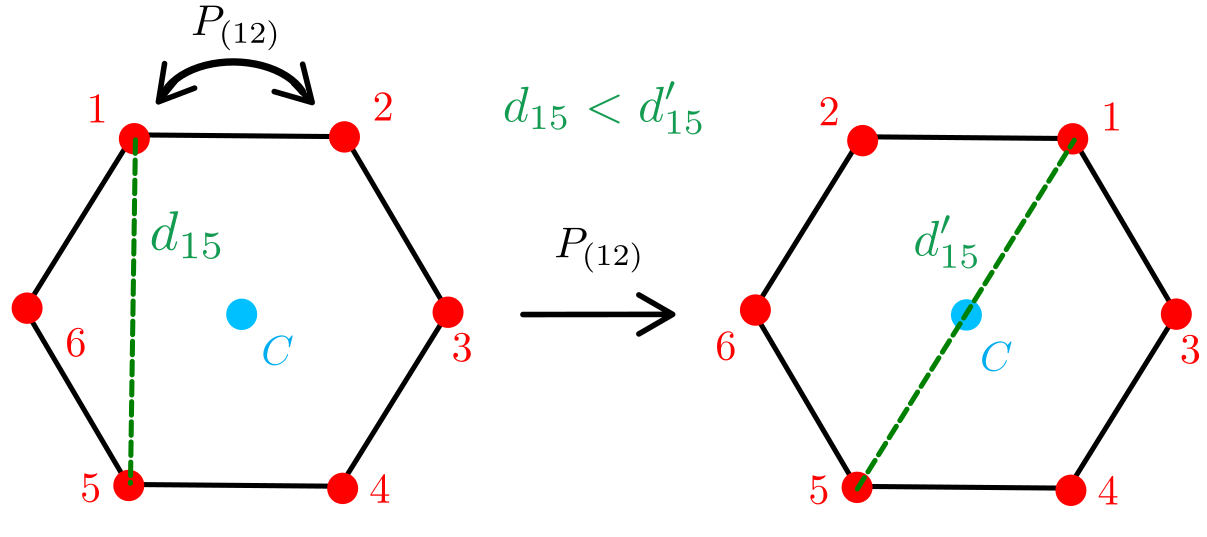
\includegraphics[width=0.8\linewidth]{fig/hexagon_perm_12.png}
\caption{Illustration of a non-isometric operation: the permutation \(P_{(12)}\).}
\label{fig:hexagon_perm_12}
\end{figure}

Although \(P_{(12)}\) can be regarded as an element of the permutation group of the hexagon’s vertices, it holds little relevance in the context of Solid-State Physics. The spatial symmetries of physical interest are isometries, which preserve distances in Euclidean space, and these are always associated with the orthogonal group \(O(n)\).

\begin{definition}[\textbf{Orthogonal group}] \label{def:orthogonal_group}
The \textit{orthogonal group} \(O(n)\) consists of all transformations of an \(n\)-dimensional Euclidean space that preserve a fixed point. In a chosen basis, these transformations can be explicitly represented as orthogonal matrices acting on \(\mathbb{R}^n\).
\begin{equation} \label{eq:O(n)}
O(n) = \qty{A: \mathbb{R}^n \to \mathbb{R}^n \mid A A^T = \1}.
\end{equation}
\end{definition}


The symmetries that constitute \(D_6\) in Example \ref{ex:symm_elems_hexagon_D6_example} form a subgroup of \(O(2)\), the group of orthogonal transformations in two-dimensional space. In the context of Condensed Matter Physics, the most relevant systems are those associated with the symmetries of point groups.
\begin{definition}[\textbf{Point group}] \label{def:point_group}
A \textit{point group} is a group of transformations acting on Euclidean space such that all symmetry operations leave a fixed point unchanged. If the origin of the coordinate system is taken as the fixed point, a point group in \(n\) dimensions can be defined as a subgroup of \(O(n)\). Each element \(M\) of a point group is either a rotation (\(\det M = 1\)) or a reflection, inversion, or improper rotation (\(\det M = -1\)). When considering only point groups that are compatible with crystals, i.e., those consistent with the symmetry constraints imposed by lattice translations, these are referred to as \textit{crystallographic point groups}.

There are $10$ crystallographic point groups in two dimensions and $32$ in three dimensions.
\end{definition}

To capture all the symmetries of a crystal, we must combine the point group operations with translations, which gives rise to the concept of a space group.

\begin{definition}[\textbf{Space group}] \label{def:space_group}
The combination of point group operations and translations that map a crystal onto itself forms the so-called \textit{space group}. Formally, a space group \(G\) in \(n\)-dimensions consists of elements \(g = \{R \mid \tau\}: \mathbb{R}^n \to \mathbb{R}^n\), where \(R \in O(n)\) represents a \textit{crystallographic} point group operation, \(\tau \in \mathbb{R}^n\) is a translation vector, and the action of $\{R \mid \tau\}$ is given by
\begin{equation} \label{eq:space_group_action_def}
\{R \mid \tau\} \r = R \r + \tau, \quad \r \in \mathbb{R}^n.
\end{equation}
In two dimensions (2D), there are 17 space groups, also known as \textit{wallpaper groups}, 10 crystallographic point groups, and 5 Bravais lattices. In three dimensions (3D), these numbers increase to 230 space groups, 32 crystallographic point groups, and 14 Bravais lattices.
\end{definition}


Pure rotations and pure translations are special cases of space group operations:
\begin{itemize}
\item $\sg{E}{0} =$ identity.
\item $\sg{R}{0} =$ pure point group operation.
\item $\sg{E}{\tau} =$ pure translation.
\end{itemize}

The result for the multiplication of two space group operations is
$$
\sg{R_2}{\tau_2} \sg{R_1}{\tau_1} \r = \sg{R_2}{\tau_2} (R_1 \r + \tau_1) =
R_2(R_1 \r + \tau_1) + \tau_2 \implies
$$
\begin{equation} \label{eq:multiplication_two_space_group_elements}
\sg{R_2}{\tau_2} \sg{R_1}{\tau_1} = \sg{R_2 R_1}{R_2\tau_1 + \tau_2}.
\end{equation}

\begin{definition}[\textbf{Standard representation for space groups}] \label{def:matrixrep_spacegroup}
We define the \textit{standard representation} for a space group $G$ by
\begin{equation} \label{eq:spacegroup-rep}
\sg{R}{\tau} =
\begin{pmatrix}
1 & 0 \\
\tau & R
\end{pmatrix},
\end{equation}
where $0$ is a row of three zeros, $\tau$ is a column vector and $R \in O(3)$. The multiplication of matrices preserve the space group structure:
\begin{equation} \label{eq:multiplication_two_space_group_elements_matrix}
\sg{R_2}{\tau_2} \sg{R_1}{\tau_1} =
\begin{pmatrix}
1 & 0 \\
\tau_2 & R_2
\end{pmatrix}
\begin{pmatrix}
1 & 0 \\
\tau_1 & R_1
\end{pmatrix} =
\begin{pmatrix}
1 & 0 \\
R_2\tau_1 + \tau_2 & R_2 R_1
\end{pmatrix} =
\sg{R_2 R_1}{R_2\tau_1 + \tau_2}.
\end{equation}
\end{definition}

\n

Notice that, although \(\{R \mid \tau\} = \{E \mid \tau\} \{R \mid 0\}\), there could be certain operations \(\{R \mid \tau\}\) where the individual elements \(\{E \mid \tau\}\) or \(\{R \mid 0\}\) do not independently belong to the space group. The two possible types of such combined operations are \textit{glide planes} and \textit{screw axes}, which are classified as \textit{nonsymmorphic} symmetries. These operations involve a fractional lattice translation combined with a reflection or a rotation, respectively.

A glide plane consists of a translation parallel to a specific plane, followed by a reflection in that plane. For instance, as shown in Figure \ref{fig:glideplane_screwaxis_a}, a fractional translation of \(\frac{1}{2}a\), where \(a\) is the lattice constant, is not a symmetry operation on its own. However, when combined with a reflection, it maps every \(A\) atom to \(A'\), forming a symmetry operation.

Similarly, a screw axis combines a translation along an axis with a simultaneous rotation. In Figure \ref{fig:glideplane_screwaxis_b}, a 3-fold screw axis is depicted, consisting of a translation of \(\frac{1}{3}a\) along the axis, followed by a 3-fold right-hand rotation.

\begin{figure}[H]
\centering
\begin{subfigure}{.5\textwidth}
  \centering
  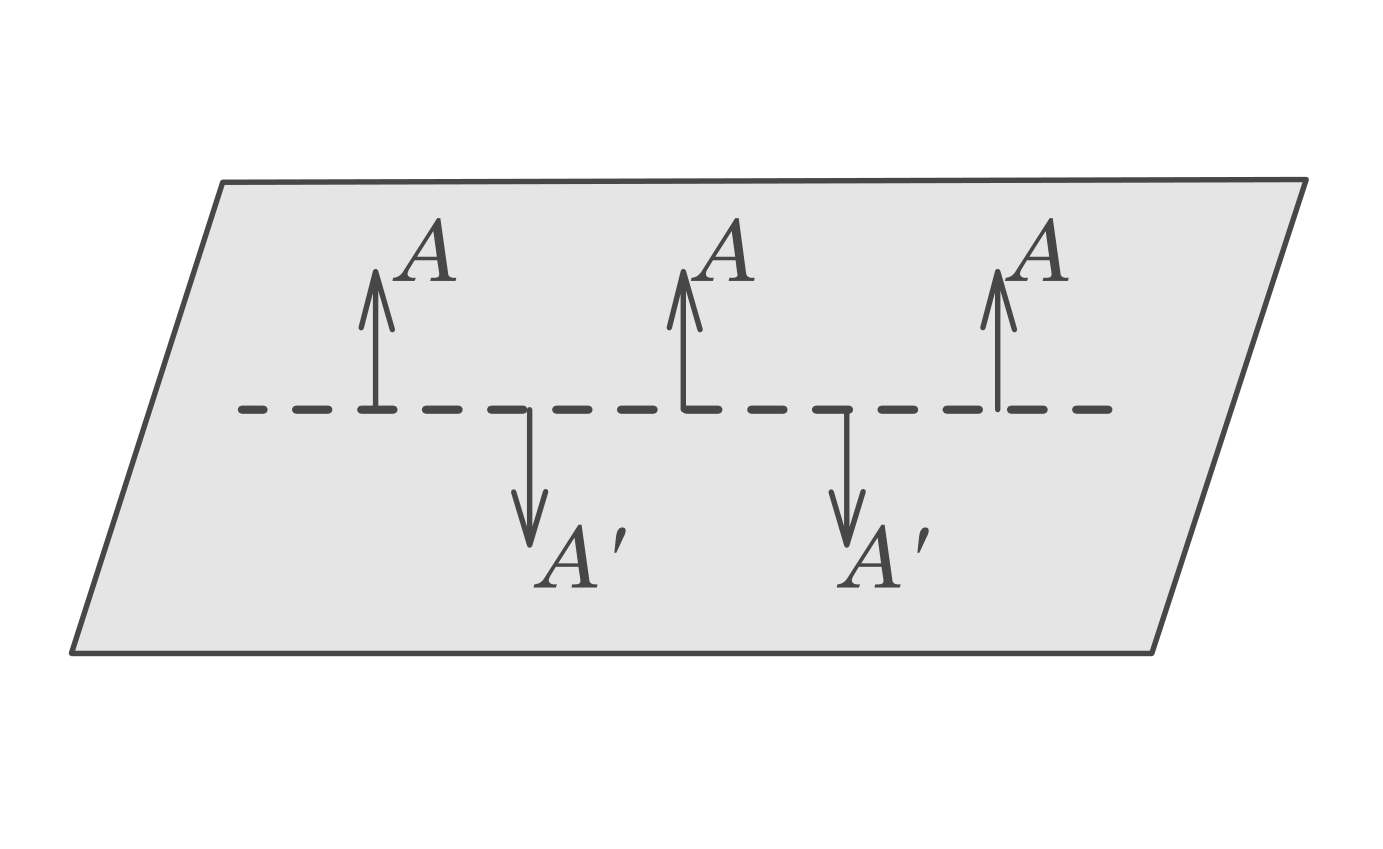
\includegraphics[height=.4\linewidth]{fig/glide_plane_dresselhaus.png}
  \caption{The glide plane takes $A$ into $A'$}
  \label{fig:glideplane_screwaxis_a}
\end{subfigure}%
\begin{subfigure}{.5\textwidth}
  \centering
  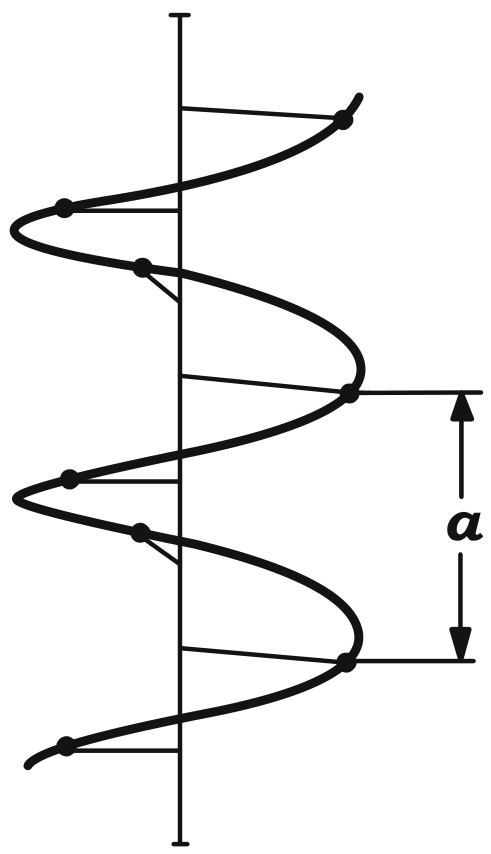
\includegraphics[height=.4\linewidth]{fig/screw_axis_dresselhaus.png}
  \caption{Right-hand threefold screw axis}
  \label{fig:glideplane_screwaxis_b}
\end{subfigure}
\caption{Illustration of a glide plane and a screw axis. Figures adapted from \cite{dresselhaus}.}
\label{fig:glideplane_screwaxis}
\end{figure}

Certain crystals possess space groups that include nonsymmorphic symmetries. Figure \ref{fig:hexagonal_ice_glideplane_a} illustrates the structure of hexagonal H$_2$O ice $I_h$, which exhibits a glide plane. Figure \ref{fig:tellurium_screwaxis_b} shows the structure of trigonal tellurium, which features a $3$-fold screw axis.
\begin{figure}[H]
\centering
\begin{subfigure}{.5\textwidth}
  \centering
  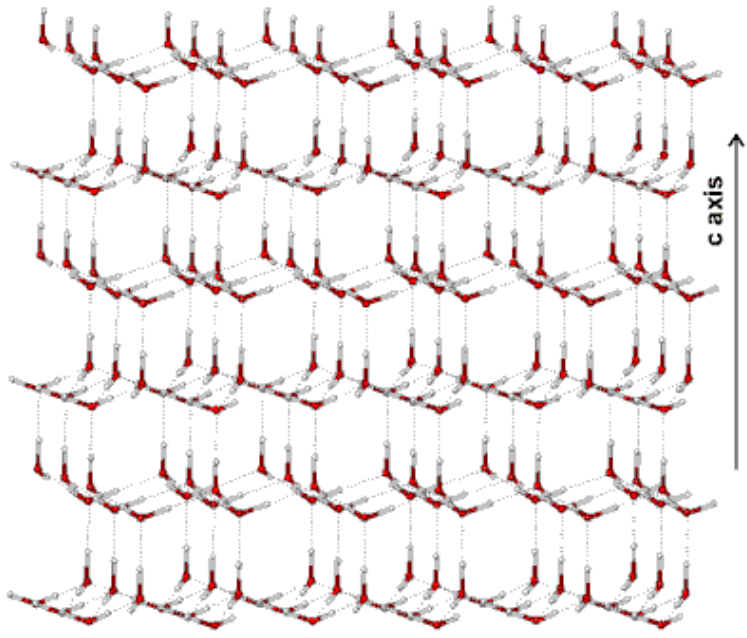
\includegraphics[height=.4\linewidth]{fig/hexagonal_ice_lattice.png}
  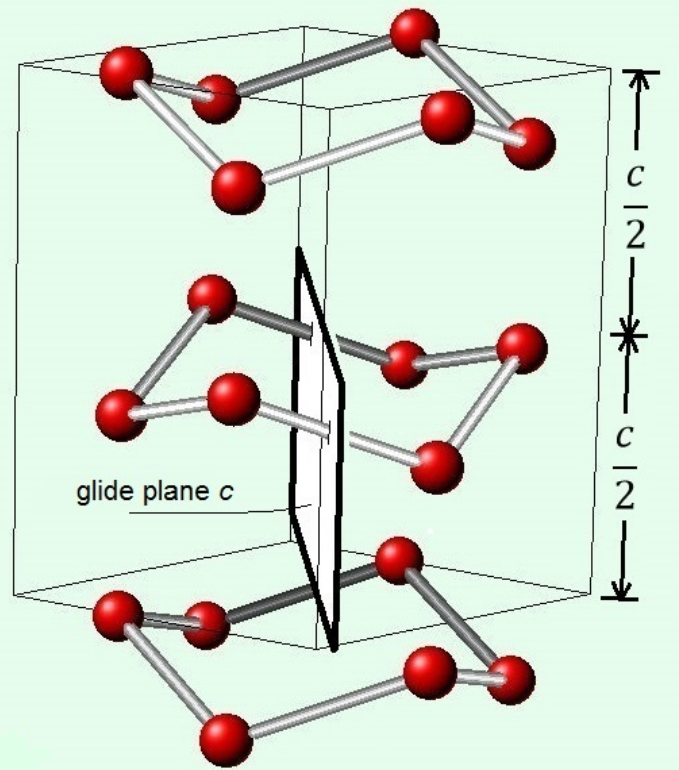
\includegraphics[height=.4\linewidth]{fig/hexagonal_ice_glide_plane.png}
  \caption{Glide plane in Hexagonal H$_2$O Ice $I_h$}
  \label{fig:hexagonal_ice_glideplane_a}
\end{subfigure}%
\begin{subfigure}{.5\textwidth}
  \centering
  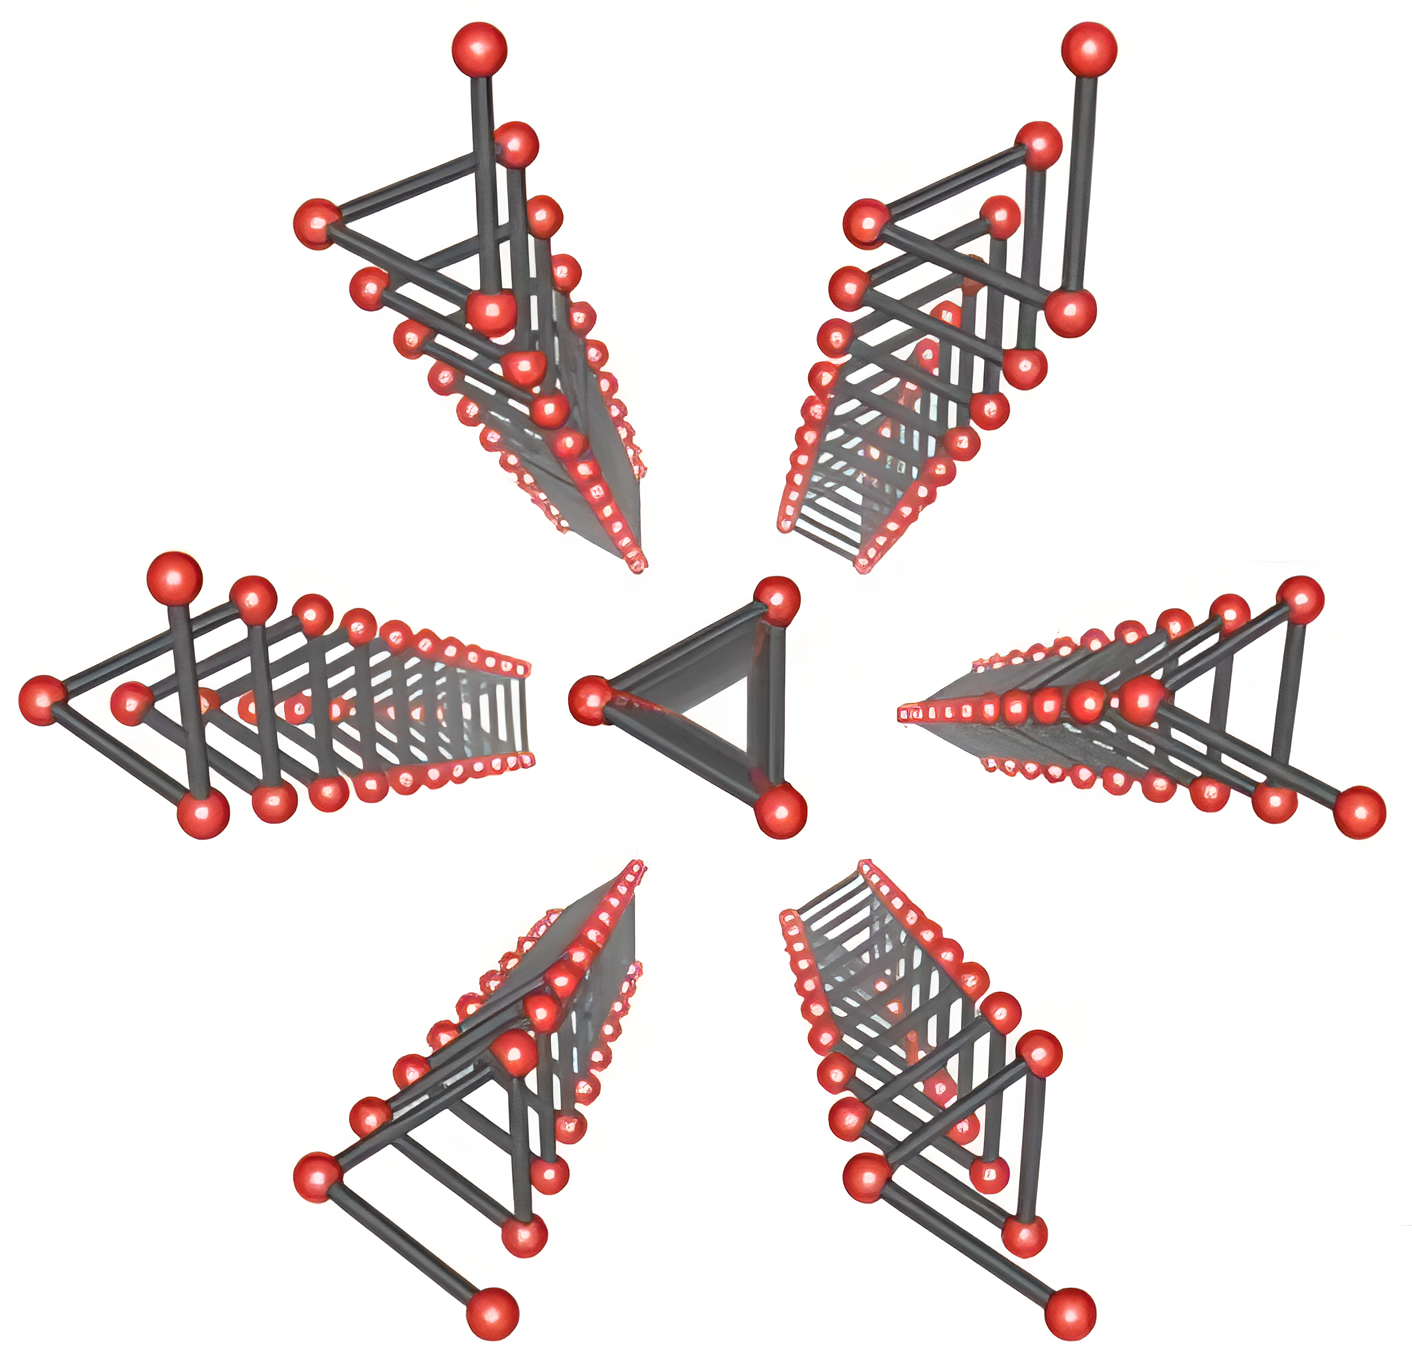
\includegraphics[height=.4\linewidth]{fig/tellurium_screw_axis_enhanced.png}  % https://overscale.imagewith.ai/
  \caption{Threefold screw axis in Trigonal Tellurium}
  \label{fig:tellurium_screwaxis_b}
\end{subfigure}
\caption{Illustration of two systems with nonsymmorphic space groups. Figures from \cite{hexagonal_ice_fig_spacegroup_wiki, hexagonal_ice_water_structure_and_science, tellurium_fig_screw_axis}.}
\label{fig:nonsymmorphic_real_systems}
\end{figure}

\begin{definition}[\textbf{Symmorphic space groups}] \label{def:symmorphic}
In a space group \(G\), its elements can always be expressed in the form
\begin{equation} \label{eq:decomp_space_group_elems_symmorphic_def}
\sg{R_\alpha}{\tau} = \sg{R_\alpha}{r_n + \tau_\alpha} = \sg{\eps}{r_n} \sg{R_\alpha}{\tau_\alpha},
\end{equation}
where \(r_n\) is a general vector of the Bravais lattice, and \(\tau_\alpha\) is either zero or a non-primitive Bravais lattice translation. Specifically, \(\tau_\alpha = 0\) corresponds to simple symmetry operations, while \(\tau_\alpha \neq 0\) corresponds to nonsymmorphic operations (glide planes or screw axes).

If, by a suitable choice of origin, all elements of \(G\) can be written in the form
\begin{equation} \label{eq:symmorphic_definition}
\sg{R_\alpha}{\tau} = \sg{R_\alpha}{r_n} = \sg{\eps}{r_n} \sg{R_\alpha}{0},
\end{equation}
where \(\tau_\alpha = 0\) for every symmetry operation, the space group \(G\) is called a \textit{symmorphic} space group. Conversely, if \(\tau_\alpha \neq 0\) for some operations, the space group is classified as \textit{nonsymmorphic}.
\end{definition}

\begin{figure}[H]
\centering
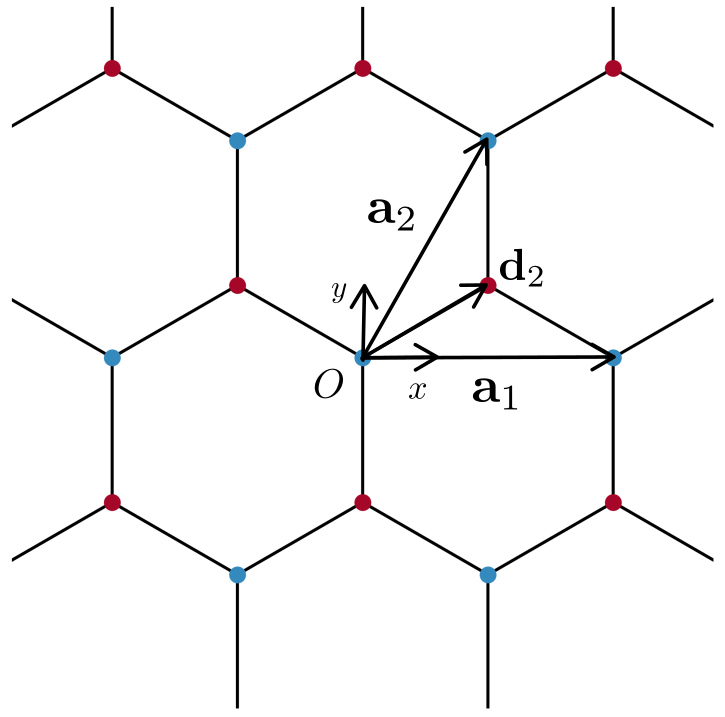
\includegraphics[width=0.55\linewidth]{fig/honeycomb_coordinates.png}
\caption{Honeycomb lattice with Bravais lattice vectors \(\mathbf{a}_1\) and \(\mathbf{a}_2\). The blue and red atoms are labeled as type $\textcolor{blue}{A}$ and type $\textcolor{red}{B}$, respectively, though they are identical.}
\label{fig:honeycomb_coordinates}
\end{figure}

\begin{figure}[H]
\centering
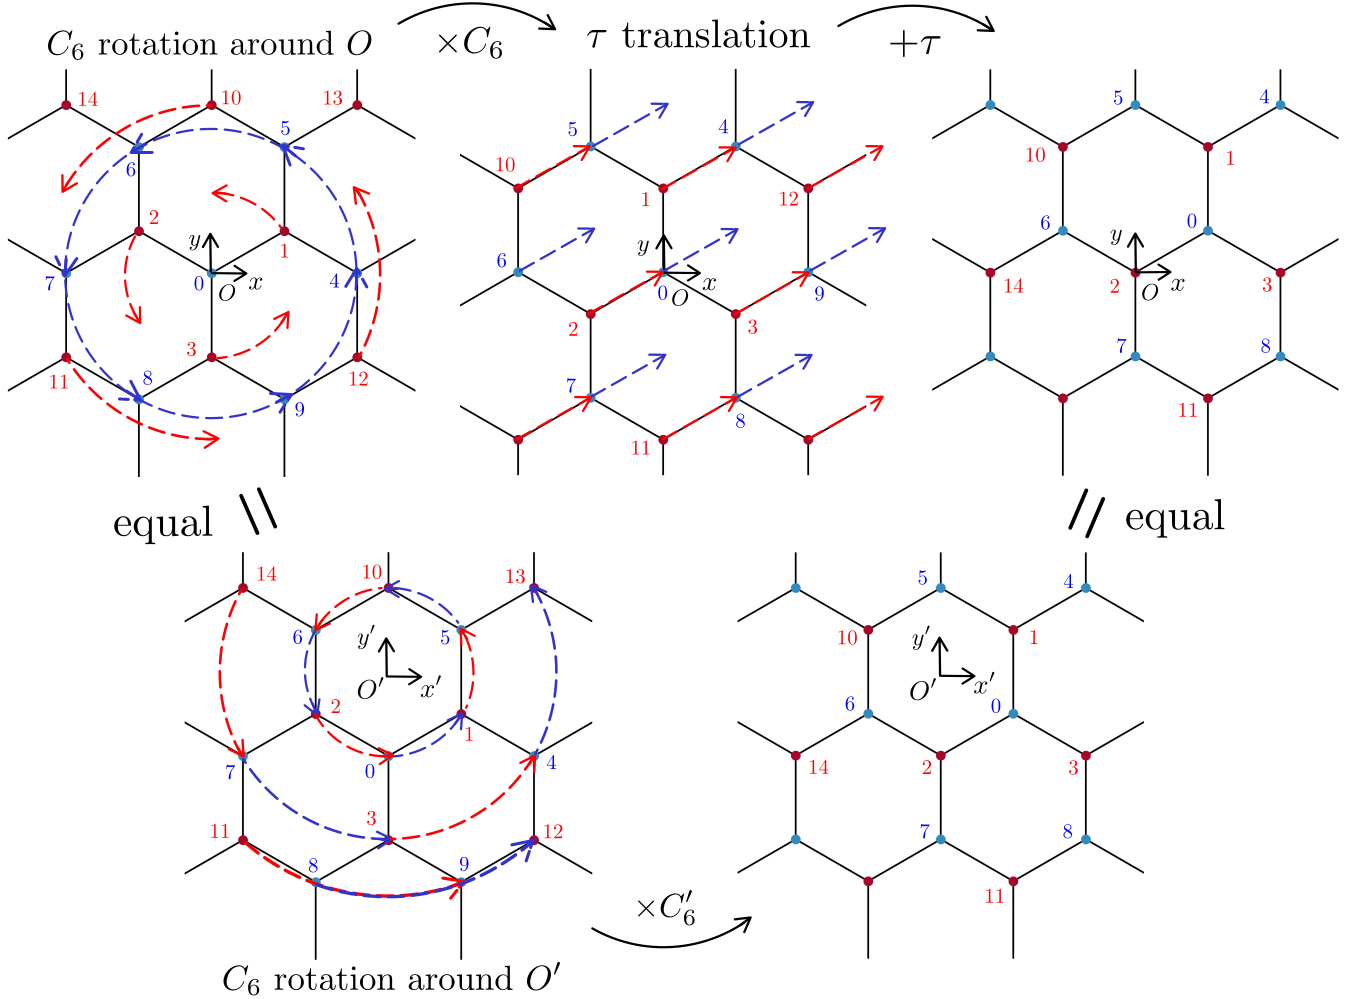
\includegraphics[width=\linewidth]{fig/space_group_example_honeycomb.png}
\caption{Illustration of Example \ref{ex:symmorphic_example_graphene}, showing a \(C_6\) rotation followed by a fractional translation \(\tau\) (top), which is equivalent to a \(C_6\) rotation around a different origin \(O'\) (bottom).}
\label{fig:space_group_example_honeycomb}
\end{figure}



\begin{example} \label{ex:symmorphic_example_graphene}
Consider the honeycomb lattice shown in Figure \ref{fig:honeycomb_coordinates}. The atoms of type \(A\) are marked in \textcolor{RoyalBlue}{blue}, and those of type \(B\) are marked in \textcolor{red}{red}. However, both types represent identical atoms (i.e., the same chemical species).

We use the Bravais lattice vectors \(\mathcal{B} = \{\vb{a}_1 = a \vu{x}, \vb{a}_2 = \frac{a}{2} \vu{x} + \frac{a\sqrt{3}}{2} \vu{y}\}\) as a vector space basis, with the origin \(O\) as indicated in Figure \ref{fig:honeycomb_coordinates}. Let \(\vb{d}_1 = \0\) and \(\vb{d}_2 = \frac{a}{2} \vu{x} + \frac{a}{2\sqrt{3}} \vu{y}\). The positions of atoms \(A\) and \(B\) are given by:
\begin{align} \label{eq:positions_atom_AB}
&& \r_A &= m_1 \vb{a}_1 + m_2 \vb{a}_2 + \vb{d}_1, \quad m_1, m_2 \in \N , & \\
&& \r_B &= n_1 \vb{a}_1 + n_2 \vb{a}_2 + \vb{d}_2, \quad \quad n_1, n_2 \in \N . &
\end{align}

Consider the space group element \(\{R \mid \tau\}\), where \(R\) is a \(60^\circ\) rotation and \(\tau = \vb{d}_2\). Its action is depicted in the upper part of Figure \ref{fig:space_group_example_honeycomb}, where the space undergoes a \(60^\circ\) rotation followed by a translation by \(\tau\). After the action of \(\{R \mid \tau\}\), although the \textcolor{RoyalBlue}{blue} and \textcolor{red}{red} colors are swapped (indicating an exchange of atoms \(A\) and \(B\)), the lattice itself (in \textbf{black}) remains unchanged. This confirms that \(\{R \mid \tau\}\) is indeed a space group symmetry. In the \(\mathcal{B}\) basis, we have:
\begin{equation} \label{eq:rotation_matrix_C6_space_group_example}
\begin{cases}
\; R \vb{a}_1 = \vb{a}_2 \\
\; R \vb{a}_2 = -\vb{a}_1 + \vb{a}_2
\end{cases}
\Rightarrow \;\;\;
R = C_6 =
\begin{pmatrix}
0 & -1 \\
1 &  1
\end{pmatrix},
\end{equation}
\begin{equation} \label{eq:tau_translation_C6_space_group_example}
\tau = \frac{1}{3} (\vb{a}_1 + \vb{a}_2) \implies
\tau =
\begin{pmatrix}
1/3 \\ 1/3
\end{pmatrix}.
\end{equation}

Observe in Figure \ref{fig:space_group_example_honeycomb} that the pure rotation \(\{R \mid 0\}\) does not preserve the lattice, nor does the pure translation \(\{E \mid \tau\}\). Moreover, as shown in Equation \ref{eq:tau_translation_C6_space_group_example}, \(\tau\) corresponds to a fractional lattice translation. At first glance, this might lead us to conclude that \(\{R \mid \tau\}\) is nonsymmorphic. However, the lower part of Figure \ref{fig:space_group_example_honeycomb} reveals that \(\{R \mid \tau\}\) is equivalent to a pure \(60^\circ\) rotation about a different origin, \(O'\). This new origin is in fact the point \(\vb{r} = OO'\) that remains fixed under the action of \(\{R \mid \tau\}\):
\begin{equation} \label{eq:fixed_point_O'_spacegroup_example}
R \r + \tau = \r \implies (R-\1) \r = -\tau \implies
\begin{pmatrix}
-1 & -1 \\
1 & 0
\end{pmatrix}
\r =
\begin{pmatrix}
-1/3 \\ -1/3
\end{pmatrix} \implies
\r =
\begin{pmatrix}
-1/3 \\ 2/3
\end{pmatrix} .
\end{equation}

This proves that \(\{R \mid \tau\}\) is a symmorphic symmetry, as it can be expressed as a rotation about a suitably chosen origin. The honeycomb lattice can be verified to correspond to a symmorphic space group: the wallpaper group \(\#17\), or equivalently, the space group \(P6mm\) (\(\#183\)).
\end{example}


%\textbf{SEI LÁ ESSE SCHRODINGER}
%
%The wave function $\psi(\r)$ of a stationary state of a quantum mechanical one-particle system with Hamiltonian $H(\r)$ satisfies the eigenvalue equation
%\begin{equation} \label{eq:schrodinger}
%H(\r) \psi(\r) = E \psi(\r),
%\end{equation}
%where $E$ is an eigenvalue of the hermitian operator $H$. If a generic transformation $g$ has been performed on the system, wavefunction and the Hamiltonian transform into $\psi(g^{-1}\r)$ and $H(g^{-1}\r)$.


%%%%%%%%%%%%%%%%%%%%%%%%%%%%%%%%%%%%%%%%%%%%%%%%%%%%%%%%%%%%%%%%%%%%%%%%%%%%%%%%%%%%%%%%%%%%%%%%%%
\section{Magnetic Space Groups} \label{sec:magnetic_space_groups}
%%%%%%%%%%%%%%%%%%%%%%%%%%%%%%%%%%%%%%%%%%%%%%%%%%%%%%%%%%%%%%%%%%%%%%%%%%%%%%%%%%%%%%%%%%%%%%%%%%

Magnetic moments in solids arise when there are unpaired electrons in electronic shells. A common example is Hund's rule, which favors the ``ferromagnetic'' interaction, leading to the appearance of an intrinsic magnetic moment. Below the ordering temperature, a magnetic structure forms, while above this temperature, the system is in a paramagnetic state.

In this section, we introduce the concept of the magnetic space group (Shubnikov group), which is crucial for studying magnetic structures. Our main focus will be to apply this theory to analyze the symmetries of the twisted bilayer graphene (TBG) system. Since TBG has negligible spin-orbit coupling (SOC) and can be considered ``spinless'', we will apply the same formalism to the sublattice degree of freedom instead of spin.

To analyze the symmetries of magnetic configurations, we introduce the time reversal operator, denoted by \(T\) or \(1'\). In the context of magnetic systems, this operator acts on magnetic moments, which are ``classical axial vectors.'' The time reversal operator reverses the direction of the electrical current, which effectively inverts the magnetic moment, as shown in Figure \ref{fig:timerev_axialvec}.

\begin{figure}[H]
\centering
\begin{subfigure}{.4\textwidth}
  \centering
  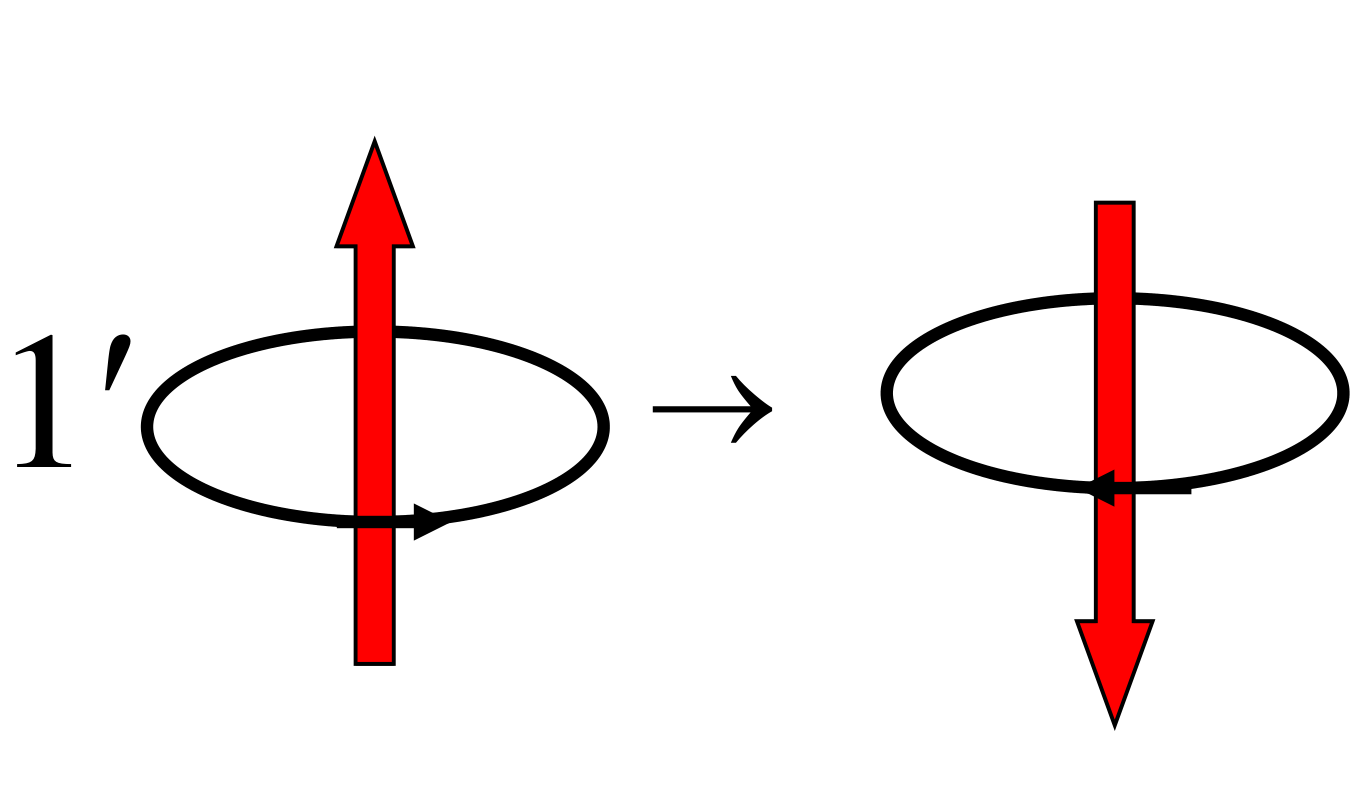
\includegraphics[height=0.6\linewidth]{fig/timerev.png}
  \caption{The time reversal operator $T = 1'$ reverses the electrical current, which inverts the magnetic moment.}
  \label{fig:timerev_a}
\end{subfigure} \hfill
\begin{subfigure}{.55\textwidth}
  \centering
  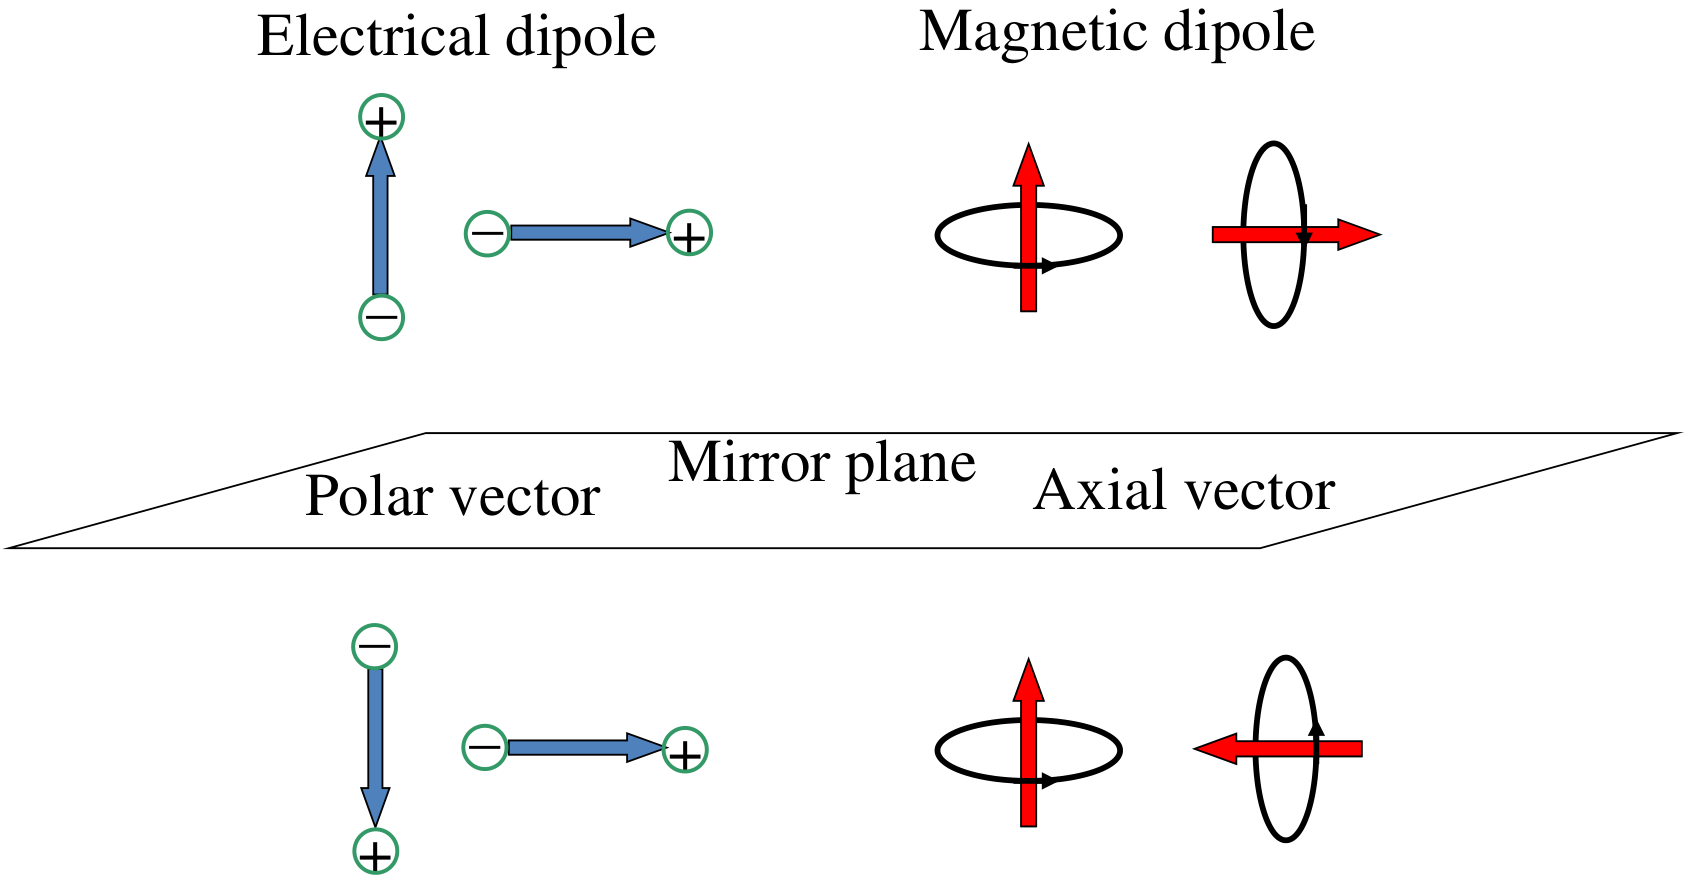
\includegraphics[width=\linewidth]{fig/axialvec.png}
  \caption{Comparison between a vector (electrical dipole) and an axial vector (magnetic dipole) under a reflection.}
  \label{fig:axialvec_b}
\end{subfigure}
\caption{The action of the time reversal operator. Figures taken from \cite{magnetic_structures2012}.}
\label{fig:timerev_axialvec}
\end{figure}

Although initially motivated by magnetic systems, the magnetic groups can be understood more abstractly as a mathematical construct: a tensor product with the group of two elements, \(\mathcal{T} = \{1, 1'\}\). In this view, time reversal is treated as an abstract operator, extending beyond its physical origins. For instance, in the context of TBG, the time-reversal operator can be interpreted as \textbf{swapping the sublattice types \(A\) and \(B\) (ISSO ESTÁ ERRADOOOO, TALVEZ EU FALE DE TIME-REVERSAL IN SPINLESS SYSTEMS)}.

Let \(G\) be a group that does not include the time-reversal operator. A \textit{magnetic group} is then defined as a subgroup of the tensor product \(G \otimes \mathcal{T}\), where its elements can be ``painted black, white, or grey,'' reflecting the interplay between time-reversal and spatial symmetries.

\begin{definition}[\textbf{Magnetic group}] \label{def:magnetic_group}
Any magnetic group \( M \) can be expressed as a subgroup of the external direct product of \( \mathcal{T} = \{1, 1'\}\) with another group \( G \) (excluding \( 1' \)), such that \( M \subseteq G \otimes \mathcal{T} \). A magnetic group $M$ is defeined to be only one of three types:
\begin{enumerate}
\item \textbf{Colorless}: These are magnetic groups of the form \(M =  G \otimes \{1\} \).

\item \textbf{Grey (Paramagnetic)}: These are the full direct product \(M = G \otimes \{1, 1'\} \).

\item \textbf{Black-and-White}: If \( H \) is a subgroup of \( G \) with \hyperref[def:left_cosets]{index} \(2\), then \( M \) is constructed as
\begin{equation} \label{eq:magnetic_black_white_def}
M = H \otimes 1 \; \cup \; (G - H) \otimes 1'.
\end{equation}
\end{enumerate}
\end{definition}

To better grasp the concept introduced in Definition \ref{def:magnetic_group}, we can draw some analogies:
\begin{enumerate}
\item Colorless groups represent systems that lack time-reversal symmetry entirely.

\item Grey groups correspond to systems in the paramagnetic state, where the temperature is above the critical ordering temperature \( T_c \). In this state, the system remains invariant under time-reversal symmetry, reflecting the absence of any net magnetic ordering.

\item Black-and-white groups can be understood as systems where, for every primed element (black), there exists a corresponding unprimed element (white). This mirrors the interplay between symmetry operations that involve time reversal and those that do not.
\end{enumerate}

The magnetic point group of the BM model of TBG is \(6'2'2\) in Hermann-Mauguin notation. In this notation, the generators of the symmetry group can be chosen as \(C_{6z} T\), \(C_{2y} T\), and \(C_{2x}\). This magnetic point group corresponds to the magnetic space group \(P6'2'2\). Understanding the symmetry operations within \(P6'2'2\) is crucial for modeling an interacting model for twisted bilayer graphene and exploring the topological phases that emerge in the system.

Figure \ref{fig:622_magnetic} illustrates the symmetries of the \(6'2'2\) magnetic point group. The black and white circles represent objects with distinct time-reversal properties, with \(+\) and \(-\) indicating the top and bottom layers, respectively. The dashed red lines indicate the \(C_2 T\) axes, which invert both the sign and the color of the circles. When \(C_{6z} T\) is applied, the circles are rotated by \(60^\circ\) around the $z$ axis, and their color is inverted as well, showcasing the combined effect of the sixfold rotation and time-reversal symmetry.


\begin{figure}[H]
\centering
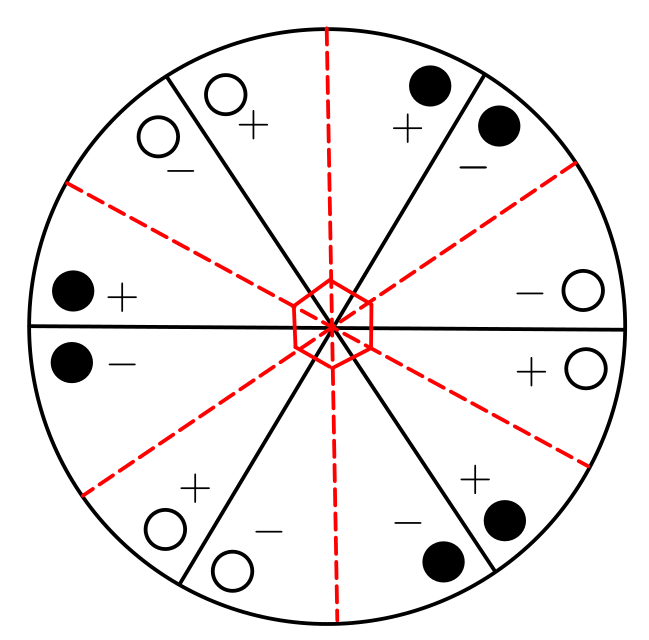
\includegraphics[width=0.5\linewidth]{fig/622_magnetic.png}
\caption{Illustration of the magnetic point group \(6'2'2\), where black and white represent time-reversal symmetry, and \(+\) and \(-\) denote different layers.}
\label{fig:622_magnetic}
\end{figure}

%\begin{example} \label{ex:magnetic_group_tbg_6'2'2}
%The magnetic point group of the BM model of TBG is $6'2'2$ in Hermann-Mauguin notation. According to the notation, we can choose its generators to be $C_{6z} T$, $C_{2y} T$ and $C_{2x}$.
%\end{example}

\section{Double groups}

Beyond the inclusion of time-reversal symmetry, which gives rise to magnetic groups, another crucial extension in symmetry analysis is the incorporation of half-integral angular momentum states, particularly relevant in systems with spin-orbit interaction. This leads to the concept of *double groups*. The one-electron Hamiltonian for a solid including spin-orbit coupling can be expressed as \cite{dresselhaus}:

\begin{equation} \label{eq:one_electron_hamiltonian_spin_orbit}
H = \underbrace{\frac{\p^2}{2m} + V(\r)}_{H_0} +
\underbrace{\frac{1}{2m^2c^2} (\grad{V} \cross \p) \vdot \vb{S}}_{H_{SO}},
\end{equation}

where \(\vb{S}\) is the spin of the electron. Here, the wave functions consist of both a spatial part and a spin part, implying that the irreducible representations used to classify states must account for spin.

Double groups emerge when dealing with systems where the total angular momentum \(j\) can take half-integral values (e.g., \(j = 1/2, 3/2, \dots\)). In such cases, the symmetry of the wave functions under rotations requires special treatment. For instance, in a free atom, which exhibits full rotational symmetry, the number of symmetry operations commuting with the Hamiltonian is infinite. Any rotation \(C_\alpha\) about an axis has a character given by \cite{dresselhaus}:

\begin{equation} \label{eq:character_chi_alpha_rotation}
\chi^{(j)}(\alpha) = \frac{\sin[(j+1/2)\alpha]}{\sin(\alpha/2)},
\end{equation}

where \(j\) is the total angular momentum and \(\alpha\) is the angle of rotation.

A key distinction arises in how the wave functions transform under a rotation of \(2\pi\). For integral angular momentum states, a \(2\pi\)-rotation acts as the identity. However, for half-integral angular momentum states, the transformation yields a sign change:

\begin{equation} \label{eq:rotation_by_2pi_half-integral}
\chi^{(j)}(\alpha+2\pi) = (-1)^{2j} \chi^{(j)}(\alpha).
\end{equation}

This sign inversion for half-integral \(j\) is a fundamental feature of spinor wave functions and motivates the concept of \textit{double groups}. Specifically, in such cases, a \(2\pi\)-rotation cannot be treated as the identity operation, as it results in a phase factor of \(-1\).

To accommodate this behavior, the double group \(\cc{G}\) is defined as an extension of the original group \(G\), where a new group element \(\cc{E}\) represents a rotation of \(2\pi\). Unlike the identity element \(E\), \(\cc{E}\) satisfies $\cc{E}^2 = E$, indicating that two successive \(2\pi\)-rotations recover the identity operation. The double group \(\cc{G}\) can thus be expressed as $\cc{G} = G \otimes \{E, \cc{E}\}$, where \(\cc{E} \v = \v\) for any three-dimensional vector \(\v\).

\begin{example} \label{ex:double_group_example}
When considering the $\cc{D}_3$ double group, its elements are doubled. Each $g \in D_3$ of them will have a corresponding barred element $\cc{g} = g \cc{E} = \cc{E} g$. Because of this, the character table of $\cc{D}_3$ is modified and will have more irreps. It can be calculated to be:

\begin{table}[H]
\caption{Character table of double group $\cc{D}_3$ (or $\cc{C}_{3v}$).}
\centering
\begin{tabular} { c c c c c c c  }
\specialrule{0.05em}{0em}{0.2em}
$\P$ & $\P E$ & $\P 2 C_3$ & $\P 3 m$ & $\P \cc{E}$ & $\P 2 \cc{C}_3$ & $\P3\cc{m}$ \\
\specialrule{0.01em}{0.2em}{0.2em}
$K_1$      & $\P1$ & $\P1$ & $\P1$  & $\P1$ & $\P1$ & $\P1$  \\
\specialrule{0.01em}{0.2em}{0.2em}
$K_2$      & $\P1$ & $\P1$ & $ -1$  & $\P1$ & $\P1$ & $ -1$  \\
\specialrule{0.01em}{0.2em}{0.2em}
$K_3$      & $\P2$ & $ -1$ & $\P0$  & $\P2$ & $ -1$ & $\P0$  \\
\specialrule{0.01em}{0.2em}{0.2em}
$\cc{K}_4$ & $\P1$ & $ -1$ & $  -i$ & $ -1$ & $\P1$ & $\P i$  \\
\specialrule{0.01em}{0.2em}{0.2em}
$\cc{K}_5$ & $\P1$ & $ -1$ & $\P i$ & $ -1$ & $\P1$ & $  -i$ \\
\specialrule{0.01em}{0.2em}{0.2em}
$\cc{K}_6$ & $\P2$ & $\P1$ & $\P0$  & $ -2$ & $ -1$ & $\P0$  \\
\specialrule{0.05em}{0.2em}{0em}
\end{tabular}
\label{tab:D3_double}
\end{table}

The irreps $K_1$, $K_2$ and $K_3$ are single-valued and correspond to irreps $A_1$, $A_2$ and $E$ of Table \ref{tab:D3}. The irreps $\cc{K}_4$, $\cc{K}_5$ and $\cc{K}_6$ are double-valued, they differentiate the identity $E$ from $\cc{E}$.

We label the irreps $K_i$, instead of the usual notation $\Gamma_i$ found at Bilbao Crystallographic Server \cite{bilbao_1}, because in Section \ref{sec:spinful_graphene} the little group at reciprocal point $K$ is isomorphic to $\cc{D}_3$, while the little group at point $\Gamma$ will be associated to $\cc{D}_6$.


\end{example}

%\begin{table}[H]
%\caption{Character table of group $\cc{D}_6$ (or $\cc{C}_{6v}$).}
%\centering
%\begin{tabular} { c c c c c c c c c c  }
%\specialrule{0.05em}{0em}{0.2em}
%$\P$ & $\P E$ & $\P 2 C_3$ & $\P2C_2$ & $\P2C_6$ & $\P6 m$ & $\P6 C_6 m$ & $\cc{E}$ & $2 \cc{C}_3$ & $2 \cc{C}_6$ \\
%\specialrule{0.01em}{0.2em}{0.2em}
%$\Gamma_1$      & $\P1$ & $\P1$ & $\P1$ & $\P1$ & $\P1$ & $\P1$ & $\P1$ & $\P1$ & $\P1$ \\
%\specialrule{0.01em}{0.2em}{0.2em}
%$\Gamma_2$      & $\P1$ & $\P1$ & $\P1$ & $\P1$ & $ -1$ & $ -1$ & $\P1$ & $\P1$ & $\P1$ \\
%\specialrule{0.01em}{0.2em}{0.2em}
%$\Gamma_3$      & $\P1$ & $\P1$ & $ -1$ & $ -1$ & $ -1$ & $\P1$ & $\P1$ & $\P1$ & $ -1$ \\
%\specialrule{0.01em}{0.2em}{0.2em}
%$\Gamma_4$      & $\P1$ & $\P1$ & $ -1$ & $ -1$ & $\P1$ & $ -1$ & $\P1$ & $\P1$ & $ -1$ \\
%\specialrule{0.01em}{0.2em}{0.2em}
%$\Gamma_5$      & $\P2$ & $ -1$ & $\P2$ & $ -1$ & $\P0$ & $\P0$ & $\P2$ & $ -1$ & $ -1$ \\
%\specialrule{0.01em}{0.2em}{0.2em}
%$\Gamma_6$      & $\P2$ & $ -1$ & $ -2$ & $\P1$ & $\P0$ & $\P0$ & $\P2$ & $ -1$ & $\P1$ \\
%\specialrule{0.01em}{0.2em}{0.2em}
%$\cc{\Gamma}_7$ & $\P2$ & $ -2$ & $\P0$ & $\P0$ & $\P0$ & $\P0$ & $ -2$ & $\P2$ & $\P0$ \\
%\specialrule{0.01em}{0.2em}{0.2em}
%$\cc{\Gamma}_8$ & $\P2$ & $\P1$ & $\P0$ & $-\sqrt{3}$ & $\P0$ & $\P0$ & $ -2$ & $ -1$ & $\P\sqrt{3}$ \\
%\specialrule{0.01em}{0.2em}{0.2em}
%$\cc{\Gamma}_9$ & $\P2$ & $\P1$ & $\P0$ & $\P\sqrt{3}$ & $\P0$ & $\P0$ & $ -2$ & $ -1$ & $-\sqrt{3}$ \\
%\specialrule{0.05em}{0.2em}{0em}
%\end{tabular}
%\label{tab:D6_double}
%\end{table}

%\begin{table}[H]
%\caption{Character table of double group $\cc{D}_2$ (or $\cc{C}_{2v}$).}
%\centering
%\begin{tabular} { c c c c c c }
%\specialrule{0.05em}{0em}{0.2em}
%$\P$ & $\P E$ & $\P 2 C_2$ & $\P 2 m$ & $\P 2 C_2 m$ & $\P \cc{E}$ \\
%\specialrule{0.01em}{0.2em}{0.2em}
%$\Gamma_1$      & $\P1$ & $\P1$ & $\P1$ & $\P1$ & $\P1$ \\
%\specialrule{0.01em}{0.2em}{0.2em}
%$\Gamma_2$      & $\P1$ & $\P1$ & $ -1$ & $ -1$ & $\P1$ \\
%\specialrule{0.01em}{0.2em}{0.2em}
%$\Gamma_3$      & $\P1$ & $ -1$ & $ -1$ & $\P1$ & $\P1$ \\
%\specialrule{0.01em}{0.2em}{0.2em}
%$\Gamma_4$      & $\P1$ & $ -1$ & $\P1$ & $ -1$ & $\P1$ \\
%\specialrule{0.01em}{0.2em}{0.2em}
%$\cc{\Gamma}_5$ & $\P2$ & $\P0$ & $\P0$ & $\P0$ & $ -2$ \\
%\specialrule{0.05em}{0.2em}{0em}
%\end{tabular}
%\label{tab:D2_double}
%\end{table}






%%%%%%%%%%%%%%%%%%%%%%%%%%%%%%%%%%%%%%%%%%%%%%%%%%%%%%%%%%%%%%%%%%%%%%%%%%%%%%%%%%%%%%%%%%%%%%%%%%
%%%%%%%%%%%%%%%%%%%%%%%%%%%%%%%%%%%%%%%%%%%%%%%%%%%%%%%%%%%%%%%%%%%%%%%%%%%%%%%%%%%%%%%%%%%%%%%%%%


%%%%%%%%%%%%%%%%%%%%%%%%%%%%%%%%% COMMENT THIS TO COMPILE main.tex %%%%%%%%%%%%%%%%%%%%%%%%%%%%%%%%
%%%-----
%%% Referências bibliográficas
%%%-----
%\addcontentsline{toc}{chapter}{\bibname}
%%\bibliographystyle{abntex2-num}
%\bibliography{citations}
%\bibliographystyle{ieeetr}
%\end{document}
%%%%%%%%%%%%%%%%%%%%%%%%%%%%%%%%% COMMENT THIS TO COMPILE main.tex %%%%%%%%%%%%%%%%%%%%%%%%%%%%%%%%
